\documentclass[11pt]{article}
\usepackage[margin=1in]{geometry}
\usepackage[T1]{fontenc}
\usepackage{lmodern}
\usepackage{amsmath,amssymb,amsthm,mathtools}
\usepackage{microtype,flafter}
\usepackage{tikz}
\usetikzlibrary{arrows.meta,positioning,calc,fit}
\usepackage[colorlinks=true,linkcolor=blue!45!black,citecolor=blue!45!black,urlcolor=blue!45!black]{hyperref}

\hypersetup{
  pdftitle={Uniform Interior C1alpha Estimates for Infinity-Harmonic Functions},
  pdfauthor={OpenAI},
  pdfsubject={Interior regularity of viscosity solutions of the infinity Laplace equation}
}
\numberwithin{equation}{section}
\allowdisplaybreaks[2]
\setlength{\emergencystretch}{2em}
\setcounter{tocdepth}{1}

\newtheorem{theorem}{Theorem}[section]
\newtheorem{proposition}[theorem]{Proposition}
\newtheorem{lemma}[theorem]{Lemma}
\newtheorem{corollary}[theorem]{Corollary}
\theoremstyle{definition}
\newtheorem{definition}[theorem]{Definition}
\theoremstyle{remark}
\newtheorem{remark}[theorem]{Remark}

\newcommand{\R}{\mathbb{R}}
\newcommand{\Dinf}{\Delta_{\infty}}
\newcommand{\Penv}{\mathcal{P}}
\newcommand{\Menv}{\mathcal{M}}
\newcommand{\Cenv}{\mathcal{C}}
\newcommand{\Senv}{\mathcal{S}}
\newcommand{\Aclass}{\mathcal{A}}
\DeclareMathOperator{\Lip}{Lip}
\DeclareMathOperator{\osc}{osc}

\title{Uniform Interior $C^{1,\alpha}$ Estimates\\
for Infinity-Harmonic Functions}
\author{OpenAI}
\date{October 4, 2026}

\begin{document}
\maketitle

\begin{abstract}
We prove a uniform interior $C^{1,\alpha_d}$ estimate for bounded
infinity-harmonic functions in every dimension $d\ge3$. For some
$\alpha_d\in(0,1/3]$ depending only on the dimension, the gradient's
supremum norm and $\alpha_d$-H\"older seminorm on $B_{1/2}$ are bounded
by a dimension-dependent constant times the oscillation on $B_1$.
The exponent is not explicit, and no endpoint or boundary regularity
claim is made. In particular, infinity-harmonic functions are locally
$C^1$ on every open subset of $\mathbb{R}^d$, for $d\ge3$.
\end{abstract}

\tableofcontents

\section{Introduction}\label{sec:introduction}

The infinity Laplace equation is associated with minimizing the largest
local Lipschitz constant. For a smooth real function on an open subset of
$\R^d$, its unnormalized operator is
\[
 \Dinf u=\langle D^2u\,\nabla u,\nabla u\rangle
       =\sum_{i,j=1}^d u_i u_j u_{ij}.
\]
Only the second derivative in the gradient direction enters the equation.
This degeneracy makes control of the full gradient a central issue even
far from the boundary. We prove a uniform interior H\"older estimate for
the gradient, with a positive exponent depending only on the dimension.

\subsection{The result}
All balls are Euclidean; $B_r$ denotes the ball centered at the origin
unless a center is specified. A continuous function $u$ on an open set
$\Omega$ is \emph{infinity-harmonic} if every local upper $C^2$ test $\phi$
at $z\in\Omega$ satisfies $\Dinf\phi(z)\ge0$, and every local lower test
satisfies $\Dinf\phi(z)\le0$. All tests are included, also when
$\nabla\phi(z)=0$. Write $\osc_Eu=\sup_Eu-\inf_Eu$, and for a vector
field $g$ set
\[
 [g]_{C^{0,\alpha}(E)}
   =\sup_{\substack{x,y\in E\\x\ne y}}
       \frac{|g(x)-g(y)|}{|x-y|^\alpha}.
\]

\begin{theorem}[Uniform interior estimate]\label{thm:main}
For every integer $d\ge3$ there are constants $\alpha_d\in(0,1/3]$ and
$C_d<\infty$ such that every bounded infinity-harmonic function
$u\in C(B_1)$, where $B_1\subset\R^d$, belongs to
$C^{1,\alpha_d}(B_{1/2})$ and satisfies
\[
 \|\nabla u\|_{L^\infty(B_{1/2})}
       +[\nabla u]_{C^{0,\alpha_d}(B_{1/2})}
       \le C_d\osc_{B_1}u.
\]
\end{theorem}

The exponent arises from a compactness argument and is not explicit.
The qualitative interior regularity statement follows on any open domain.

\begin{corollary}[Interior $C^1$ regularity]\label{cor:interior-c1}
Let $d\ge3$, let $\Omega\subseteq\R^d$ be a nonempty connected open set,
and let $u\in C(\Omega)$ be infinity-harmonic. Then
$u\in C^1_{\mathrm{loc}}(\Omega)$.
\end{corollary}

\begin{proof}
For each $x_0\in\Omega$, choose $r>0$ with
$\overline B_{2r}(x_0)\subset\Omega$. Continuity bounds $u$ on this closed
ball, and $y\mapsto u(x_0+2ry)$ is infinity-harmonic on $B_1$.
Theorem~\ref{thm:main} applies and gives the conclusion near $x_0$.
\end{proof}

More precisely, the same change of variables gives
\[
 \|\nabla u\|_{L^\infty(B_r(x_0))}
   +r^{\alpha_d}[\nabla u]_{C^{0,\alpha_d}(B_r(x_0))}
   \le \frac{C_d}{r}\osc_{B_{2r}(x_0)}u,
\]
after enlarging $C_d$ if necessary.

\subsection{Context and methods}
Aronsson's work on absolute minimization connects the infinity Laplace
equation with a local version of the optimal Lipschitz extension problem
\cite{Aronsson1967}. A locally Lipschitz function $u$ is an absolute
minimizer if, for every open $V\Subset\Omega$ and every Lipschitz
competitor $w$ with $w=u$ on $\partial V$,
\[
  \|Du\|_{L^\infty(V)}\le\|Dw\|_{L^\infty(V)}.
\]
Aronsson identified the equation for smooth absolute minimizers.
Jensen established its viscosity characterization and uniqueness for the
Dirichlet problem \cite{Jensen1993}. Crandall, Evans, and Gariepy
developed the equivalent comparison-with-cones formulation and the
associated local slope estimates \cite{CrandallEvansGariepy2001}.
These results supply a robust theory of continuous solutions, while
regularity beyond local Lipschitz continuity presents a separate
difficulty: the equation controls second derivatives only in the gradient
direction.

The first-order regularity theory separates affine approximation from
uniqueness and continuity of the approximating slope. Building on the
cone and slope framework of Crandall, Evans, and Gariepy,
Crandall and Evans proved that infinitesimal blow-ups at a fixed point
are affine \cite{CrandallEvansGariepy2001,CrandallEvans2001}.
Savin proved continuity of the gradient in the plane
\cite{Savin2005}, and Evans and Savin obtained planar interior
$C^{1,\alpha}$ estimates for some positive universal exponent
\cite{EvansSavin2008}. Evans and Smart subsequently proved
differentiability at every point in every dimension
\cite{EvansSmart2011}. Their conclusion identifies a unique derivative
at each point; continuity of that derivative is a further assertion.
For a significant higher-dimensional special class, Peng, Zhang, and
Zhou proved interior $C^1$ regularity and nonvanishing of the gradient for
infinity-harmonic potentials in convex rings
\cite{PengZhangZhou2025}.

The planar endpoint has also been the subject of recent work. Brustad's
June 2026 preprint proves local $1/3$-H\"older continuity of the gradient
under the additional assumptions that it never vanishes and has a
Lipschitz inverse \cite[Theorem~1.1]{Brustad2026}.
Xu's July 2026 preprint states the unrestricted planar
$C^{1,1/3}_{\mathrm{loc}}$ theorem
\cite[Theorem~1.1]{Xu2026}; it separately leaves open a universal
endpoint norm estimate \cite[Remark~1.5(i)]{Xu2026}.
The theorem proved here concerns uniform interior estimates for arbitrary
solutions in dimensions $d\ge3$.

The restriction to an exponent at most $1/3$ is natural. Aronsson's
example \cite{Aronsson1984}
\[
  u(x)=|x_1|^{4/3}-|x_2|^{4/3},\qquad x\in\R^d,
\]
is infinity-harmonic and has
$|Du(he_1)-Du(0)|=\tfrac43|h|^{1/3}$.
It therefore rules out any exponent greater than $1/3$, in every
dimension $d\ge2$. Our compactness argument produces a positive exponent
depending on the dimension and does not identify the endpoint value.

\subsection{Proof strategy}
The proof has two parts. First we reduce failure of a uniform power
rate for affine approximation to an entire nonaffine solution of a
limiting equation. Then we prove that the estimates inherited by
that limit force it to be affine.

Normalize the original solutions to have oscillation at most one and
adjoin a linear coordinate, $U(y,b)=u(y)+b$. This preserves the equation
and ensures that accurate affine fits have nonzero slopes. A three-point
estimate controls the midpoint defect of a function close to an affine
function, divided by the endpoint separation, uniformly even at much
smaller separations. Combined with fixed-center affine blow-ups, it
gives affine approximation with error $o(r)$ uniformly across normalized
solutions and interior centers. This small-scale uniformity is essential:
compactness of the solutions alone would not give a common rate for
their derivatives.

We measure finer approximation on cylinders with axial radius $r$ and
transverse radius $\sqrt\lambda r$, allowing error $\lambda r$ from an
affine function whose slope points along the axis. A power rate of decay
for the worst fitting parameter makes consecutive slopes converge at a
uniform power rate, giving the gradient estimate. If every power bound
fails, a selection of almost-maximal normalized errors provides scales
with two properties: one fitting parameter fails at the selected center,
but a fixed multiple of it succeeds at every nearby center and every
fixed multiple of that scale. Those fits provide compactness after
stretching the transverse variables and magnifying the deviation from
the central affine fit.

The entire limit $v(x,t)$, with $x\in\R^d$ and $t\in\R$, satisfies
\[
 F[v]:=D^2v[(\nabla_xv,1)]=0,
 \qquad D^2v[\xi]=\xi^{\mathsf T}D^2v\,\xi.
\]
At every center $(x,t)$ and radius $R>0$ it admits coefficients
$p\in\R^d$ and $q\in\R$ such that
\[
 |v(x+h,t+\ell)-v(x,t)-p\cdot h-q\ell|\le C_0R
 \quad\text{if } |\ell|\le R,\quad |h-p\ell|\le R,
\]
with one finite constant $C_0$. The horizontal slope determines the
shear of the fitting box. Our Liouville Theorem states that every entire
solution with these fits is affine. An affine limit would improve the
selected failed fit, proving the desired power bound.

The anisotropic scaling and the limiting equation are due to Evans and
Savin \cite[Sections~2.3--2.4]{EvansSavin2008}. Their argument derives
gradient H\"older regularity from quantitative flatness estimates in thin
cylinders; the estimates required for that argument are established in
their paper in dimension two. Quadratic comparisons on horizontal slices
and monotone forward and backward slopes also appear in their analysis
\cite[Section~3]{EvansSavin2008}. Here uniform affine approximation,
comparison of intersecting cylinders, and a Liouville theorem for an
entire class with affine fits at every center and scale provide the
compactness argument. The Liouville proof combines an extremal
horizontal averaging defect, preservation of the subsolution inequality
by its variance-penalized envelope, and localization of contacts at
arbitrarily small times around a common terminal point.

For the Liouville argument, introduce, for $\ell>0$, the quadratic envelopes
\begin{align*}
 \Penv_\ell v(x,t)
   &=\sup_y\left\{v(y,t+\ell)-\frac{|y-x|^2}{2\ell}\right\},
 \\
 \Menv_\ell v(x,t)
   &=\inf_y\left\{v(y,t-\ell)+\frac{|y-x|^2}{2\ell}\right\}.
\end{align*}
The fits give subquadratic spatial growth, so the extrema are attained.
The quotients $(\Penv_\ell v-v)/\ell$ and
$(v-\Menv_\ell v)/\ell$ are nondecreasing in $\ell$ and have a common
small-length limit at each point. If both quotients were constant in
length at one point, quadratic comparison would force $v$ to be affine.
We seek such a limit while retaining an obstruction to affinity.

That obstruction is a horizontal Jensen defect: the excess of a weighted
average of values over the value at their spatial mean. Starting from one
nonaffine solution, we recenter and rescale configurations for which the
ratio of the defect to the root mean square distance from the mean
approaches its supremum.
Compactness then gives an extremal solution. For $t>0$, take the supremum
of these averages at time $t$ and a fixed spatial mean, after subtracting
their variance divided by $2t$. The extremal ratio bounds the resulting
barycentric envelope's excess over $v$ by a fixed multiple of time, with
equality at a selected point. Subtracting that linear function of time produces a subsolution
$W\le v$ touching $v$ at positive time; the unshifted envelope has a
strictly positive gap there. The variance penalty is affine along the
directions in the viscosity test, which makes the subsolution inequality
survive this averaging.

Forward optimizers for $W$ and backward optimizers for $v$ define two
possible steps from each space-time point. A fair choice between them
gives a drift inequality controlling the expected sum of squared discrepancies
of their velocities from a common reference velocity. This control is
unchanged by a fitted change of frame. It yields contacts at decreasing
positive times, with one terminal point remaining in a bounded part of
infinitely many fitted frames. The common small-length envelope slope at
that point is finite. After normalization at these shrinking contact
scales, every fixed envelope length corresponds to a length tending to zero
at the same terminal point. Differences of the normalized slopes cancel
the affine correction and tend to zero. A further limit therefore has
constant envelope slopes at every length, yet retains the positive
barycentric gap.
Rigidity gives the contradiction.

Section~\ref{sec:flatness} proves the lift, slope, and three-point estimates.
Section~\ref{sec:reduction} proves Theorem~\ref{thm:main} from the
Liouville Theorem. Sections~\ref{sec:limiting-tools}
and~\ref{sec:envelope-contact} construct the envelopes and extremal contact.
Sections~\ref{sec:discrete-propagation}
and~\ref{sec:contact-localization} propagate and localize that contact.
Section~\ref{sec:rigidity} proves rigidity and completes the Liouville
argument.

Throughout, equations with positive second-order sign use the same
viscosity convention as $\Dinf$: subsolutions satisfy the nonnegative
inequality at upper tests, and supersolutions the nonpositive inequality
at lower tests. Tests for equations in $(x,t)$ involve all variables
together. For a symmetric matrix $A$, we write $A[\xi]=\xi^{\mathsf T}A\xi$.

\section{Uniform local flatness}\label{sec:flatness}

This section proves the local estimates used to obtain uniform affine approximation in Section~\ref{sec:reduction}. The decisive estimate controls midpoint defects at every separation, including separations much smaller than the scale on which a function is known to be close to an affine function.

\subsection{A linear lift and affine blow-ups}

\begin{lemma}\label{lem:linear-lift}
If $u$ is infinity-harmonic in $\Omega\subseteq\R^d$, then
\[
  U(y,b)=u(y)+b
\]
is infinity-harmonic in $\Omega\times\R$.
\end{lemma}

\begin{proof}
Suppose that $\phi$ touches $U$ from above at $(y_0,b_0)$. Restriction to the vertical line gives $\phi_b(y_0,b_0)=1$. Put $p=\nabla_y\phi(y_0,b_0)$. If $p\ne0$, choose an affine function $\ell$ with $\ell(y_0)=b_0$ and $\nabla\ell\cdot p=1$. The function
\[
  \psi(y)=\phi(y,\ell(y))-\ell(y)
\]
touches $u$ from above at $y_0$. At that point $\nabla\psi=p$, because $\phi_b=1$, and
\[
  D^2\psi[p]
  =\phi_{yy}[p]+2\phi_{yb}\cdot p+\phi_{bb}
  =D^2\phi[(p,1)]=\Dinf\phi.
\]
The viscosity inequality for $u$ gives the required sign. If $p=0$, the vertical upper contact gives $\phi_{bb}\ge0$, and this is $\Dinf\phi$ because $\nabla\phi=(0,1)$. Lower tests are identical with the inequalities reversed.
\end{proof}

We recall the cone comparison and slope estimates of Crandall, Evans, and Gariepy \cite{CrandallEvansGariepy2001}. These give local Lipschitz regularity and the information about blow-ups used here. For an infinity-harmonic function $w$ on an open set $D\subseteq\R^n$, define, whenever $\overline B_r(z)\subset D$,
\[
  L_r^\pm(w;z)=\frac1r\max_{|h|\le r}\bigl\{\pm(w(z+h)-w(z))\bigr\}.
\]

\begin{lemma}\label{lem:cone-slopes}
The function $w$ is locally Lipschitz. For a fixed center $z$, both $L_r^+(w;z)$ and $L_r^-(w;z)$ are nondecreasing in $r$. For each fixed allowable radius, they are continuous as functions of the center.
\end{lemma}

\begin{proof}
Fix $\overline B_r(z)\subset D$ and $L>L_r^+(w;z)$. Choose $\gamma>0$ so small that
\[
  \gamma r<L-L_r^+(w;z),\qquad 2\gamma r<L.
\]
On $\partial B_r(z)$ the function $w$ lies strictly below
\[
  w(z)+L|Z-z|-\gamma|Z-z|^2.
\]
It lies below this function throughout the ball. Otherwise the positive maximum of their difference is attained at an interior point different from $z$, and the displayed function, shifted by a constant, is an upper test there. Writing $\rho=|Z-z|$, its infinity Laplacian is
\[
  -2\gamma(L-2\gamma\rho)^2<0,
\]
contrary to the viscosity inequality. Letting $\gamma\downarrow0$ and then $L\downarrow L_r^+(w;z)$ gives
\[
  w(Z)-w(z)\le L_r^+(w;z)|Z-z|\qquad (Z\in\overline B_r(z)).
\]
Applying the same argument to $-w$ gives the lower bound with $L_r^-(w;z)$. These bounds prove monotonicity in the radius.

For centers in a compact neighborhood, choose one small radius whose balls remain in $D$. The two slopes at that radius are uniformly bounded by the oscillation on a larger compact set divided by the radius. The preceding inequalities then give a common local Lipschitz bound. Continuity in the center at fixed radius follows from uniform continuity of $w$ on a compact neighborhood, taking the maximum over the fixed set $\{|h|\le r\}$.
\end{proof}

For the following fixed-center affine blow-up result, see Crandall, Evans, and Gariepy \cite{CrandallEvansGariepy2001} and Crandall and Evans \cite[pp.~124--127]{CrandallEvans2001}; we include a variant of the latter cone-slope argument.

\begin{proposition}[Affine blow-ups at a fixed center]\label{prop:affine-blowups}
Let $w$ be infinity-harmonic in $D$ and let $z\in D$. Every locally uniform limit, along a sequence $r_i\downarrow0$, of
\[
  V_i(Y)=\frac{w(z+r_iY)-w(z)}{r_i}
\]
is a linear function on $\R^n$. Such limits exist after passage to subsequences.
\end{proposition}

\begin{proof}
The local Lipschitz bound and the exhaustion of $\R^n$ by the rescaled domains give subsequential convergence on compact sets. By Lemma~\ref{lem:cone-slopes}, the finite limits
\[
  L_*^\pm=\lim_{r\downarrow0}L_r^\pm(w;z)
\]
exist. They are equal. Indeed, if $h_r$ attains the positive maximum, then for each fixed small $R>r$, once $r$ is sufficiently small,
\[
  L_r^+(w;z)\le L_r^-(w;z+h_r)\le L_R^-(w;z+h_r).
\]
First let $r\downarrow0$, using continuity at fixed $R$ and $|h_r|\le r$, and then let $R\downarrow0$. This gives $L_*^+\le L_*^-$. Reversing signs gives equality; write the common value as $L_*$.

Let $V$ be a limit. Uniform convergence on balls shows that
\[
  L_R^+(V;0)=L_R^-(V;0)=L_*\qquad(R>0),
\]
and that the slopes at every other center retain monotonicity in their radius. In particular $|V(Y)|\le L_*|Y|$. For any center $q$,
\[
  L_T^\pm(V;q)\le\frac{L_*(T+|q|)+|V(q)|}{T}.
\]
For a fixed radius at $q$, bound its slope by the slope at $T$ and send $T\to\infty$. Thus every slope of $V$ is at most $L_*$, so $V$ is globally $L_*$-Lipschitz.

If $L_*=0$, then $V=0$. Otherwise let $x_R$ and $y_S$ attain the positive and negative extrema on the balls of radii $R$ and $S$ centered at zero. The equality of the origin slopes gives
\[
  L_*(R+S)=V(x_R)-V(y_S)
     \le L_*|x_R-y_S|\le L_*(R+S).
\]
Equality throughout forces $|x_R|=R$, $|y_S|=S$, and these points to lie on opposite rays of one line. Comparing all choices of $R,S$ gives a unit vector $e$ such that $V(te)=L_*t$ for every real $t$. The Lipschitz bound then yields
\[
  L_*t-L_*|Y-te|\le V(Y)\le L_*t+L_*|Y-te|.
\]
Letting $t\to+\infty$ in the lower bound and $t\to-\infty$ in the upper bound gives $V(Y)=L_*e\cdot Y$.
\end{proof}

This argument establishes the linearity of each blow-up without requiring uniqueness of its slope. The stronger everywhere differentiability theorem is due to Evans and Smart \cite{EvansSmart2011}.

\subsection{The three-point estimate}

We use one standard viscosity tool. For a continuous function $g$, its second-order superjet $J^{2,+}g(z)$ consists of pairs $(p,X)$ for which
\[
  g(z+h)\le g(z)+p\cdot h+\tfrac12X[h]+o(|h|^2).
\]
The closed superjet $\overline J^{2,+}g(z)$ consists of limits of such jets at points approaching $z$, with the function values also converging. For the continuous operators used here, the viscosity inequality at upper tests applies to closed superjets as well.

\begin{lemma}[Theorem of sums, {\cite[Theorem~3.2]{CIL1992}}]\label{lem:sum-rule}
Let $g_j$ be continuous on open subsets of Euclidean spaces. Suppose that $\sum_{j=1}^N g_j(z_j)-\Psi(z_1,\ldots,z_N)$ has a local maximum at an interior product point, where $\Psi$ is $C^2$ near that point. Set $A=D^2\Psi$. For every $\eta>0$ there are symmetric matrices $X_j$ such that
\[
  (D_j\Psi,X_j)\in\overline J^{2,+}g_j(z_j),\qquad
  \operatorname{diag}(X_1,\ldots,X_N)\le A+\eta A^2.
\]
\end{lemma}

\begin{proposition}[Three-point flatness]\label{prop:three-point}
Let $U_i$ be infinity-harmonic on $B_1\subset\R^n$ with a common Lipschitz bound, and let $\ell_i$ be affine functions such that
\[
  \|U_i-\ell_i\|_{L^\infty(B_1)}\longrightarrow0.
\]
Then
\begin{equation}\label{eq:three-point}
  \sup_{\substack{x,y\in B_{1/4}\\x\ne y}}
  \frac{|U_i(x)+U_i(y)-2U_i((x+y)/2)|}{|x-y|}
  \longrightarrow0.
\end{equation}
\end{proposition}

\begin{proof}
Put $w_i=U_i-\ell_i$ and $\varepsilon_i=\|w_i\|_{L^\infty(B_1)}$. The slopes of $\ell_i$ are bounded: evaluating at $e/2$ and $-e/2$ for every unit vector $e$ gives $|\nabla\ell_i\cdot e|\le\Lip(U_i)+2\varepsilon_i$. Thus $w_i$ have a common Lipschitz bound $C$.

Suppose that \eqref{eq:three-point} fails. Passing to a subsequence and replacing $U_i,\ell_i$ by their negatives if necessary, there are endpoint pairs in $B_{1/4}$ with positive midpoint defect greater than $\delta|x-y|$ for some fixed $\delta>0$. For triples $x,y,z\in\overline B_{3/4}$ with $x\ne y$, write
\[
  c=\frac{x+y}{2},\qquad h=z-c,\qquad r=|x-y|,
  \qquad f(r)=r-\frac18r^{3/2}.
\]
Here $0<r\le3/2$, so $\nu r\le f(r)\le r$ with $\nu=1-\sqrt{3/2}/8>0$. Choose a smooth function $B(c)$ that equals $\delta/2$ on $\overline B_{1/4}$, is at least $\delta/2$ everywhere, and equals a sufficiently large constant $B_{\mathrm{out}}$ when $|c|\ge1/2$. Consider
\begin{equation}\label{eq:three-point-maximum}
  w_i(x)+w_i(y)-2w_i(z)-B(c)f(r)-\frac{|h|^2}{r^2}.
\end{equation}
Allowing the third point to move permits the use of Lemma~\ref{lem:sum-rule}, while the quadratic penalty keeps it close to the midpoint. The factor $B(c)$ localizes the maximum, and the concavity of $f$ will supply the dominant negative second variation.
The violating pair with $z=c$ makes this expression positive. On the other hand it is at most
\[
  Cr+2C|h|-B(c)f(r)-\frac{|h|^2}{r^2}
  \le Cr+C^2r^2-B(c)f(r).
\]
Its upper limit as $r\downarrow0$ is therefore at most zero, uniformly in the other variables. A positive maximum is attained at some triple with $r>0$.

At these maximizing triples, $r\to0$ as $i\to\infty$: positivity and $Bf\ge\delta\nu r/2$ give $r\le8\varepsilon_i/(\delta\nu)$. Comparing the maximizing value with the admissible choice $z=c$ also gives
\[
  \frac{|h|^2}{r^2}\le2\bigl(w_i(c)-w_i(z)\bigr)\le2C|h|,
  \qquad |h|\le2Cr^2.
\]
Choose $B_{\mathrm{out}}>(C+\tfrac32C^2)/\nu$. The preceding upper bound for \eqref{eq:three-point-maximum} is then nonpositive when $|c|\ge1/2$. Hence $|c|<1/2$ at a positive maximum. Since $r\to0$ and $h=O(r^2)$, the maximizing triples are interior to $(B_{3/4})^3$ for all large $i$.

At one such triple set $q=\nabla\ell_i$ and $e=(x-y)/r$. Apply Lemma~\ref{lem:sum-rule} to the functions $U_i,U_i,-2U_i$ and the test
\[
  \Psi=\ell_i(x)+\ell_i(y)-2\ell_i(z)+B(c)f(r)+\frac{|h|^2}{r^2}.
\]
This test is $C^2$ near the triple. Define $p_1=D_x\Psi$, $p_2=D_y\Psi$, and $p_0=-D_z\Psi/2$. Direct differentiation gives
\begin{align*}
  p_1&=q+\tfrac12f(r)DB(c)-h/r^2+a e,\\
  p_2&=q+\tfrac12f(r)DB(c)-h/r^2-a e,\\
  p_0&=q-h/r^2,\qquad
  a=B(c)f'(r)-2|h|^2/r^3.
\end{align*}
These vectors and $a$ are bounded. Since $f'(r)=1-3\sqrt r/16$ and $|h|=O(r^2)$, we also have $a\ge\delta/4$ for all sufficiently large $i$.

Let $\sigma=(p_1,p_2,p_0)$. The third jet supplied by Lemma~\ref{lem:sum-rule} has gradient $-2p_0$. The function $-2U_i$ is infinity-harmonic, so the viscosity inequalities for the three superjets give
\[
  X_1[p_1]\ge0,\qquad X_2[p_2]\ge0,\qquad X_3[-2p_0]\ge0.
\]
In particular $X_3[p_0]\ge0$. If $A=D^2\Psi$ at the maximum, the matrix inequality evaluated at $\sigma$ gives
\[
  0\le\operatorname{diag}(X_1,X_2,X_3)[\sigma]
       \le A[\sigma]+\eta|A\sigma|^2.
\]
The maximum, $A$, and $\sigma$ are fixed while $\eta\downarrow0$, although the jets may vary. It follows that $A[\sigma]\ge0$.

We compute the same quadratic form by moving $(x,y,z)$ along the straight line with velocity $\sigma$ and parameter $\tau$, with $\tau=0$ at the maximum. The endpoint relative velocity $p_1-p_2=2ae$ is parallel to $x-y$, and the third velocity differs from the mean endpoint velocity by $O(r)$. Write $c(\tau),h(\tau),r(\tau)$ for the induced quantities, and use dots for their derivatives at zero. The formulas above give
\[
  \dot r=2a,\qquad \ddot r=0,\qquad
  \dot c=\tfrac12(p_1+p_2)=O(1),\qquad
  \dot h=p_0-\dot c=-\tfrac12f(r)DB(c)=O(r).
\]
Since $h=O(r^2)$,
\[
  \left.\frac{d^2}{d\tau^2}\frac{|h(\tau)|^2}{r(\tau)^2}\right|_{\tau=0}
  =\frac{2|\dot h|^2}{r^2}
   -\frac{8\dot r\,h\cdot\dot h}{r^3}
   +\frac{6\dot r^{\,2}|h|^2}{r^4}=O(1).
\]
Also $f''(r)=-3/(32\sqrt r)$, and therefore
\begin{align*}
  \left.\frac{d^2}{d\tau^2}\bigl(B(c(\tau))f(r(\tau))\bigr)\right|_{\tau=0}
  &=B(c)f''(r)\dot r^{\,2}+2f'(r)\dot r\,DB(c)\cdot\dot c\\
  &\quad+f(r)D^2B(c)[\dot c]\\
  &=-\frac{3B(c)a^2}{8\sqrt r}+O(1)\longrightarrow-\infty.
\end{align*}
The affine part of $\Psi$ has zero Hessian. Thus $A[\sigma]\to-\infty$, contradicting its nonnegativity and proving \eqref{eq:three-point}.
\end{proof}

The three-point estimate is uniform over every nonzero endpoint separation.
This allows the observation scale and the scale of affine approximation
to tend to zero at different rates. Lemma~\ref{lem:family-flatness} uses
that freedom to obtain affine approximation uniformly over the full
normalized family of solutions and all interior centers.

\section{Uniform power decay and the gradient estimate}\label{sec:reduction}

We now prove the estimate in Theorem~\ref{thm:main}, conditional on a Liouville Theorem whose proof occupies the remaining sections. The argument works with all normalized solutions at once. We first obtain a common modulus of affine approximation, then use anisotropic compactness to force a power rate. Fits at this rate give the H\"older estimate for the gradient. The scaling and limiting equation also occur in Evans and Savin \cite[Sections~2.3--2.4]{EvansSavin2008}.

\begin{theorem}[Liouville Theorem]\label{thm:liouville}
Let $m\ge1$ and $0\le C_0<\infty$. Suppose that $v\in C(\R^m\times\R)$ is a viscosity solution of
\begin{equation}\label{eq:limit-pde}
  F[v]:=D^2v[(\nabla_xv,1)]=0.
\end{equation}
Suppose, in addition, that for every $z=(x,t)\in\R^m\times\R$ and every $R>0$ there are $p\in\R^m$ and $a\in\R$ such that
\begin{equation}\label{eq:limit-fit}
  \left|v(x+h,t+\ell)-v(x,t)-p\cdot h
       -\left(a-\frac{|p|^2}{2}\right)\ell\right|\le C_0R
  \quad\text{if }\quad |\ell|\le R,\quad |h-p\ell|\le R.
\end{equation}
Then $v$ is affine.
\end{theorem}

We prove Theorem~\ref{thm:liouville} in Sections~\ref{sec:limiting-tools}--\ref{sec:rigidity}. For clarity, a pair $(p,a)$ satisfying \eqref{eq:limit-fit} will be called a \emph{fit at $z$ of radius $R$}. Its domain is the sheared box
\[
  Q_R(z;p)=\{(x+h,t+\ell): |\ell|\le R,\ |h-p\ell|\le R\}.
\]
The ordinary time coefficient of the fitted affine function is $q=a-|p|^2/2$. We use $(p,a)$ because a sheared change of frame acts by subtracting the frame parameters, as shown in Section~\ref{sec:limiting-tools}.

\subsection{A flatness modulus for the normalized family}

Fix $d\ge3$, put $n=d+1$, and write $B_r^k$ for the ball of radius $r$ centered at zero in $\R^k$. Let $\mathcal U$ be the family of all functions
\[
  U(y,b)=u(y)+b\qquad ((y,b)\in B_1^d\times\R),
\]
where $u$ is a continuous infinity-harmonic function with
$u(0)=0$ and $\osc_{B_1^d}u\le1$. By Lemma~\ref{lem:linear-lift}, each $U$ is infinity-harmonic. The family is uniformly bounded and has a common Lipschitz constant $L$ on $\overline B_{7/8}^n$. Indeed, $|u|\le1$, and the oscillations of the lifts are uniformly bounded on $\overline B_{15/16}^n$. At every center in $\overline B_{7/8}^n$, Lemma~\ref{lem:cone-slopes} bounds both slopes of radius $1/16$ by that common oscillation divided by $1/16$. This gives a common Lipschitz bound for nearby pairs; subdividing a segment gives the bound for all pairs in the ball. All constants in this section, unless indexed by additional parameters, depend only on $d$.

Set
\[
  G=B_{3/4}^n,\qquad D(z)=\operatorname{dist}(z,\partial G),
\]
and denote the added unit direction by $e_b$. For $P\ne0$, $0<\lambda<1$, and $r>0$, put $N_P=P/|P|$ and define the closed cylinder
\[
  Z_\lambda(z,r;P)
   =\{z+h: |h\cdot N_P|\le r,\quad
               |h-(h\cdot N_P)N_P|\le\sqrt\lambda r\}.
\]
For $U\in\mathcal U$, $z\in G$, and $0<r\le D(z)/8$, call $\lambda$ \emph{good for $U$ at $(z,r)$} if some $P\ne0$ satisfies
\begin{equation}\label{eq:physical-fit}
  |U(Z)-U(z)-P\cdot(Z-z)|\le\lambda r
       \qquad (Z\in Z_\lambda(z,r;P)).
\end{equation}
We call this a cylinder fit. Its cylinder is contained in $B_{2r}(z)\subset G$. Let $\beta_U(z,r)$ be the supremum of the parameters in $(0,1)$ that are not good, with value zero if there are none, and set
\begin{equation}\label{eq:flatness-function}
  b(s)=\sup\{\beta_U(z,r):U\in\mathcal U,\ z\in G,
                        \ 0<r\le sD(z)\},\qquad 0<s\le1/8.
\end{equation}
Thus $0\le b\le1$ and $b$ is nondecreasing. Goodness itself need not be monotone in $\lambda$. The supremum definition ensures that every parameter in $(\beta_U(z,r),1)$ is good.

\begin{lemma}[Uniform qualitative flatness]\label{lem:family-flatness}
The family modulus in \eqref{eq:flatness-function} satisfies
\begin{equation}\label{eq:family-flatness}
  b(s)\longrightarrow0\qquad(s\downarrow0).
\end{equation}
Every cylinder fit satisfies
\begin{equation}\label{eq:physical-slope-bounds}
  |P|\le L+\sqrt\lambda,\qquad
  |P\cdot e_b-1|\le\sqrt\lambda.
\end{equation}
\end{lemma}

\begin{proof}
The cylinder contains $\overline B_{\sqrt\lambda r}(z)$. Evaluating the fit on this ball and using the Lipschitz bound gives the first inequality in \eqref{eq:physical-slope-bounds}. The exact increment of $U$ in direction $e_b$ equals the increment length, which gives the second.

Suppose that \eqref{eq:family-flatness} fails. There are $s_i\to0$, functions $U_i\in\mathcal U$, centers $z_i\in G$, radii $0<r_i\le s_iD(z_i)$, and parameters $\lambda_i$ that are not good at these triples, with $\lambda_i\ge\delta>0$. Passing to a subsequence, the common bounds give
\[
  z_i\longrightarrow z_*\in\overline G,\qquad
  U_i\longrightarrow U_\circ
       \quad\hbox{uniformly on }\overline B_{7/8}^n.
\]
The limit $U_\circ$ is infinity-harmonic on $B_{7/8}^n$ by the usual viscosity stability argument \cite[Section~6]{CIL1992}: add a positive fourth-order term to an upper test to make its contact strict, take nearby interior maxima for the approximating functions minus that test, and pass their inequalities to the limit. The added term leaves the first two derivatives at contact unchanged. A negative fourth-order term and minima treat lower tests. This argument also applies to the varying continuous jet operators below, since they converge uniformly on compact jet sets. Choose scales $R_i\downarrow0$ so slowly that
\begin{equation}\label{eq:slow-scales}
  r_i+|z_i-z_*|+
    \|U_i-U_\circ\|_{L^\infty(\overline B_{7/8}^n)}=o(R_i).
\end{equation}
Such a decreasing sequence can be obtained after passage to a subsequence, since all three terms tend to zero. The point $z_*$ is interior to $B_{7/8}^n$. Proposition~\ref{prop:affine-blowups}, applied to the one function $U_\circ$ at $z_*$, gives a further subsequence on which its $R_i$ blow-ups converge locally uniformly to a linear function. By \eqref{eq:slow-scales}, the functions
\[
  \widehat U_i(X)=
    \frac{U_i(z_*+R_iX)-U_i(z_*)}{R_i}
\]
converge to that same linear function uniformly on $B_1^n$. They are infinity-harmonic and uniformly Lipschitz there. Proposition~\ref{prop:three-point} therefore gives numbers $\varepsilon_i\to0$ such that
\begin{equation}\label{eq:slow-scale-midpoint}
  |\widehat U_i(X)+\widehat U_i(Y)
       -2\widehat U_i((X+Y)/2)|\le\varepsilon_i|X-Y|
       \qquad (X,Y\in B_{1/4}^n).
\end{equation}

Return now to the smaller radii $r_i$. The functions
\[
  W_i(H)=\frac{U_i(z_i+r_iH)-U_i(z_i)}{r_i}
\]
are uniformly bounded and Lipschitz on $\overline B_2^n$, so a further subsequence converges uniformly there to $W$. The slow-scale choice ensures that $z_i+r_i\overline B_2^n\subset B_{R_i/4}(z_*)$ for all large $i$. Substituting
\[
  X=\frac{z_i-z_*+r_iH}{R_i},\qquad
  Y=\frac{z_i-z_*+r_iK}{R_i}
\]
into \eqref{eq:slow-scale-midpoint} shows that the midpoint defect of $W_i$ is at most $\varepsilon_i|H-K|$. Thus $W$ satisfies the midpoint identity on $\overline B_2^n$. Continuity and dyadic subdivision on segments make $W$ affine on this ball. Since $W(0)=0$ and $W(e_b)=1$, it has the form $W(H)=P\cdot H$ with $P\cdot e_b=1$.

Uniform convergence now gives, for all large $i$,
\[
  \sup_{|H|\le2}|U_i(z_i+r_iH)-U_i(z_i)-r_iP\cdot H|
       <\delta r_i.
\]
The nonzero slope $P$ therefore gives a fit with error at most $\lambda_i r_i$ on $Z_{\lambda_i}(z_i,r_i;P)\subset B_{2r_i}(z_i)$. This contradicts the choice of $\lambda_i$ and proves \eqref{eq:family-flatness}.
\end{proof}

The larger scales $R_i$ allow a varying sequence of solutions to be compared with a blow-up of one limit function. The three-point estimate then transfers flatness back to the possibly much smaller scales $r_i$. No uniform differentiability theorem for the original family is used.

\subsection{Selection of scales}

Our next objective is a power bound for the single modulus $b$, which already takes the supremum over all normalized solutions.

\begin{proposition}[Uniform power decay]\label{prop:power-decay}
Assume Theorem~\ref{thm:liouville}. There are $B\in(0,\infty)$, $\gamma\in(0,1]$, and $s_0\in(0,1/8]$, depending only on $d$, such that
\begin{equation}\label{eq:power-decay}
  b(s)\le Bs^\gamma\qquad(0<s\le s_0).
\end{equation}
\end{proposition}

We prove this proposition by contradiction. Its failure means that $b(s)/s^\gamma$ is unbounded near zero for every $\gamma>0$. The next lemma selects scales where this failure occurs, while obtaining a slightly enlarged good parameter uniformly at nearby centers and radii.

\begin{lemma}\label{lem:bad-scales}
Suppose that \eqref{eq:power-decay} fails for every positive exponent. There are $\gamma_i\downarrow0$, $s_i\downarrow0$, functions $U_i\in\mathcal U$, centers $z_i\in G$, radii $0<r_i\le s_iD(z_i)$, and parameters $\lambda_i\downarrow0$ such that $\lambda_i$ is not good for $U_i$ at $(z_i,r_i)$ and the following holds. Set $\Lambda=32$. For every fixed $M\ge2$, for all sufficiently large $i$, every center $z$ with $|z-z_i|\le Mr_i$ and radius $0<r\le Mr_i$ are admissible, and $\Lambda\lambda_i$ is good for $U_i$ at $(z,r)$.
\end{lemma}

\begin{proof}
Choose any sequence $\gamma_i\downarrow0$. The function $b(s)s^{-\gamma_i}$ is bounded on intervals separated from zero and is unbounded near zero. Taking a factor-two approximate maximum on a sufficiently long truncated interval $[h_i,1/8]$ gives a point $s_i$ such that $s_i\to0$ and
\begin{equation}\label{eq:running-maximum}
  \frac{b(s)}{s^{\gamma_i}}
     \le2\frac{b(s_i)}{s_i^{\gamma_i}}\qquad(s_i\le s\le1/8).
\end{equation}
For example, make the approximate maximum larger than the supremum on $[1/i,1/8]$ to ensure $s_i<1/i$. Pass to a subsequence to make $s_i$ decreasing. We have $b(s_i)>0$. Choose $U_i\in\mathcal U$, $z_i\in G$, and $r_i\le s_iD(z_i)$ with $\beta_{U_i}(z_i,r_i)>b(s_i)/2$, and then choose a parameter $\lambda_i>\beta_{U_i}(z_i,r_i)/2$ that is not good for $U_i$ at this center and radius. This uses only approximate suprema and gives
\begin{equation}\label{eq:bad-parameter}
  b(s_i)/4<\lambda_i\le b(s_i).
\end{equation}
In particular $\lambda_i\to0$; pass to a further subsequence if needed to make it decreasing.

Fix $M\ge2$. For large $i$, we have $Mr_i\le Ms_iD(z_i)<D(z_i)$, so every $z$ with $|z-z_i|\le Mr_i$ belongs to $G$. The distance to the boundary then satisfies
\[
  D(z)\ge D(z_i)-Mr_i\ge\tfrac12D(z_i)>0.
\]
For $r\le Mr_i$ we have $r/D(z)\le2Ms_i\le1/8$, so the center and radius are admissible. By \eqref{eq:running-maximum} and \eqref{eq:bad-parameter}, uniformly over all these choices,
\[
  \beta_{U_i}(z,r)\le b(2Ms_i)
     \le2b(s_i)(2M)^{\gamma_i}
     \le8\lambda_i(2M)^{\gamma_i}
     <32\lambda_i<1
\]
for all sufficiently large $i$. Here $(2M)^{\gamma_i}\to1$ for each fixed $M$, so the same $\Lambda=32$ works for every fixed $M$; only the threshold in $i$ depends on $M$. The parameter $\Lambda\lambda_i$ is strictly greater than every bad parameter and is therefore good.
\end{proof}

We isolate the geometry used to compare fitted slopes. It is a statement about affine fits and does not use the equation. When $\theta^2=\Lambda\lambda_i$, the rescaling below divides transverse slope errors by $\sqrt{\lambda_i}$ and longitudinal errors by $\lambda_i$. The $O(\theta)$ direction estimate controls the normalized transverse coefficient, while the $O(\theta^2)$ norm estimate, together with the quadratic angular error, controls the normalized longitudinal coefficient.

\begin{lemma}[Comparison of cylinder fits]\label{lem:cylinder-comparison}
Fix $0<c_*\le C_*<\infty$. Suppose two fits for the same function, of the form \eqref{eq:physical-fit}, with parameter $\theta^2\in(0,1)$, have slopes $P,P'$ satisfying $c_*\le |P|,|P'|\le C_*$. Write $n=P/|P|$ and $n'=P'/|P'|$. If their centers agree and their radii are $H$ and $H'$ with $H\le H'\le2H$, then
\begin{equation}\label{eq:cylinder-comparison}
  |P-P'|+|n-n'|\le C\theta,\qquad
  \bigl||P|-|P'|\bigr|\le C\theta^2,
\end{equation}
where $C$ depends only on $c_*,C_*$. The same conclusion holds for equal radii $H$ at centers $z,z'$ if $z'$ lies in the first cylinder with axial and transverse offsets at most $H/4$ and $\theta H/4$, respectively.
\end{lemma}

\begin{proof}
In the common-center case both cylinders contain $B_{\theta H}(z)$. Evaluation of the difference of the fits on this ball gives $|P-P'|\le3\theta$. Normalization of the vectors, using the lower norm bound, gives $|n-n'|\le C\theta$. Choose a fixed small $c>0$. The point $z+cHn$ belongs to both cylinders: relative to $n'$ its transverse displacement is at most $cH|n-n'|\le Cc\theta H$, and its axial displacement is at most $cH$. Taking $c$ sufficiently small, the fit errors at that point give
\[
  |(P-P')\cdot n|\le C\theta^2.
\]
Since $1-n'\cdot n=|n-n'|^2/2$,
\[
  \bigl||P|-|P'|\bigr|
   \le |(P-P')\cdot n|+|P'|(1-n'\cdot n)\le C\theta^2.
\]

For displaced centers, a ball $B_{c\theta H}(z')$ with fixed small $c$ belongs to both cylinders by the quarter-radius margins. Subtracting the first fit's value at $z'$ makes it an estimate for increments from $z'$ with error $2\theta^2H$; the second fit has error $\theta^2H$. Evaluation on the common ball again gives the vector and direction bounds. The segment $z'+s n'$ for $|s|\le c'H$ lies in both cylinders when $c'>0$ is sufficiently small: the first cylinder's initial offsets use a quarter of its radii, and the additional transverse offset is at most $c'H|n-n'|$. Evaluation on this segment and the same norm calculation give the last bound in \eqref{eq:cylinder-comparison}.
\end{proof}

\subsection{The normalized limit}

For $U_i$ at $(z_i,r_i)$, choose a fitted slope $P_i$ for the good parameter $\Lambda\lambda_i$ of Lemma~\ref{lem:bad-scales}. Put $c_i=|P_i|$. By \eqref{eq:physical-slope-bounds}, after discarding finitely many indices,
\begin{equation}\label{eq:base-norm-bounds}
  \tfrac12\le c_i\le L+1.
\end{equation}
Use orthonormal coordinates with final unit vector $P_i/c_i$, write the transverse variable as $x\in\R^d$, and define $v_i$ by
\begin{equation}\label{eq:anisotropic-rescaling}
  U_i\bigl(z_i+r_i(\sqrt{\lambda_i}x,t)\bigr)
   =U_i(z_i)+r_i c_i\bigl(t+\lambda_i v_i(x,t)\bigr).
\end{equation}
These coordinates depend on $i$. The domains of $v_i$ exhaust $\R^d\times\R$, since $D(z_i)/r_i\ge1/s_i\to\infty$.

For a smooth test $\phi$ for $v_i$, the corresponding test for $U_i$ has gradient $c_i(\sqrt{\lambda_i}\nabla_x\phi,1+\lambda_i\phi_t)$ and Hessian
\[
  \frac{c_i}{r_i}
  \begin{pmatrix}
    D^2_{xx}\phi&\sqrt{\lambda_i}D_{xt}\phi\\
    \sqrt{\lambda_i}D_{tx}\phi&\lambda_i\phi_{tt}
  \end{pmatrix}.
\]
Consequently its infinity Laplacian is the positive factor $\lambda_i c_i^3/r_i$ times
\begin{equation}\label{eq:rescaled-pde}
  D^2\phi[(\nabla_x\phi,1+\lambda_i\phi_t)].
\end{equation}
Thus $v_i$ solve the equation obtained by setting \eqref{eq:rescaled-pde} equal to zero in the viscosity sense.

\begin{proposition}\label{prop:nonaffine-limit}
For the sequence supplied by Lemma~\ref{lem:bad-scales} and the normalization \eqref{eq:anisotropic-rescaling}, a subsequence of the $v_i$ converges locally uniformly to a nonaffine function $v\in C(\R^d\times\R)$ satisfying \eqref{eq:limit-pde} and \eqref{eq:limit-fit} with one finite constant $C_0$.
\end{proposition}

\begin{proof}
Set $\theta_i=\sqrt{\Lambda\lambda_i}$. A good fit of radius $Rr_i$ has error $\theta_i^2Rr_i$ and transverse radius $\theta_i Rr_i$. Its slope obeys uniform upper and lower norm bounds by \eqref{eq:physical-slope-bounds}, once $i$ is large enough.

For each fixed $R\ge2$, Lemma~\ref{lem:bad-scales}, applied with any fixed $M>R$, provides fits at $z_i$ through successive doublings from $r_i$, followed if necessary by a final step to $Rr_i$ of ratio at most two, for all sufficiently large $i$. Comparing them by Lemma~\ref{lem:cylinder-comparison} gives, for a slope $P_R$ at the latter radius and its unit vector $n_R$,
\begin{equation}\label{eq:base-cylinder-comparison}
  |n_R-P_i/c_i|\le C\theta_i(1+\log R),\qquad
  \bigl||P_R|-c_i\bigr|\le C\theta_i^2(1+\log R).
\end{equation}
Fix a box $|x|,|t|\le K$ in the coordinates of \eqref{eq:anisotropic-rescaling} and a radius factor $S>0$. Choose $R\ge2$ so large that $R>16K$ and
\[
  K\bigl(\Lambda^{-1/2}+C(1+\log R)\bigr)<R/4.
\]
Such a choice is possible because $R/\log R\to\infty$. Next fix $M>\max\{2,2K,R,S\}$. The physical centers in the box are within $2Kr_i$ of $z_i$, and all radii in the comparisons below are at most $\max\{R,S\}r_i$. Lemma~\ref{lem:bad-scales} therefore supplies these fits uniformly once $i$ is sufficiently large. The physical image of the box then lies inside the cylinder at $z_i$ for $P_R$, with axial and transverse offsets at most one quarter of the respective radii. For the axial offset use $|\sqrt{\lambda_i}x|+|t|\le2K$. For the transverse offset, \eqref{eq:base-cylinder-comparison} gives the bound
\[
  K\bigl(\sqrt{\lambda_i}+C\theta_i(1+\log R)\bigr)<\theta_i R/4
\]
in units of $r_i$.

Compare a fit centered at any point of this box, first at radius $Rr_i$ with the enclosing fit, and then through successive doublings or halvings, with a final ratio at most two, to radius $Sr_i$. The number of comparisons depends on $K,S$ but not on $i$. If $P=(P_x,P_t)$ is any such slope in the coordinates of \eqref{eq:anisotropic-rescaling}, Lemma~\ref{lem:cylinder-comparison} gives
\[
  |P/|P|-P_i/c_i|\le C_{K,S}\theta_i,
  \qquad \bigl||P|-c_i\bigr|\le C_{K,S}\theta_i^2.
\]
Since $P_i/c_i$ is the last coordinate vector,
\[
  |P_x|\le C_{K,S}\theta_i,\qquad
  |P_t-c_i|\le\bigl||P|-c_i\bigr|
      +\tfrac12|P|\,|P/|P|-P_i/c_i|^2
      \le C_{K,S}\theta_i^2.
\]
It follows that the normalized coefficients
\begin{equation}\label{eq:normalized-fit-slopes}
  p_i'=\frac{P_x}{c_i\sqrt{\lambda_i}},\qquad
  q_i'=\frac{P_t/c_i-1}{\lambda_i}
  \quad\text{satisfy}\quad |p_i'|+|q_i'|\le C_{K,S}.
\end{equation}
In particular, using the enclosing fit at $z_i$ in \eqref{eq:anisotropic-rescaling} gives on the box
\[
  |v_i(x,t)-p_{i,R}'\cdot x-q_{i,R}'t|\le\Lambda R/c_i.
\]
Thus $v_i$ are uniformly bounded on each fixed box.

We next express the domain of a fit in these coordinates. Suppress the index $i$ temporarily, write $\lambda=\lambda_i$, and set
\[
  A=1+\lambda q_i',\qquad N=(A^2+\lambda|p_i'|^2)^{1/2},
  \qquad n=\frac{(\sqrt\lambda p_i',A)}{N}.
\]
For fixed $K,S$, \eqref{eq:normalized-fit-slopes} gives $A>0$, $N/A=1+O_{K,S}(\lambda)$, and $|n_x|=O_{K,S}(\sqrt\lambda)$ for large $i$. The physical axis has ratio $\sqrt\lambda\,p_i'/A$ of transverse to axial displacement, which becomes the finite shear $p_i'/A$ after the transverse stretch. Figure~\ref{fig:anisotropic-fit} illustrates this change of geometry. The next calculation identifies a sheared box contained in the cylinder's image in normalized coordinates, with a fixed margin at the cylinder's axial ends. The exact decomposition
\begin{equation}\label{eq:cylinder-shear-decomposition}
  (\sqrt\lambda h,\ell)
   =\frac{\ell N}{A}\,n
       +\left(\sqrt\lambda\left(h-\frac{p_i'}A\ell\right),0\right)
\end{equation}
shows that the mapped increment lies in the radius-$Sr_i$ cylinder whenever
\begin{equation}\label{eq:normalized-fit-domain}
  |\ell|\le S/2,\qquad \left|h-\frac{p_i'}A\ell\right|\le S,
\end{equation}
for all large $i$. Indeed the residual in \eqref{eq:cylinder-shear-decomposition} has transverse projection at most $\sqrt\lambda S\le\theta_i S$, and its axial projection is $O_{K,S}(\lambda S)$. The first term has axial length at most $(1+O_{K,S}(\lambda))S/2$, leaving a strict axial margin. Dividing \eqref{eq:physical-fit} by $r_i c_i\lambda_i$ therefore gives
\begin{equation}\label{eq:normalized-fit}
  |v_i(x+h,t+\ell)-v_i(x,t)-p_i'\cdot h-q_i'\ell|
      \le\frac{\Lambda}{c_i}S
\end{equation}
on \eqref{eq:normalized-fit-domain}. The coefficient of $S$ is independent of $K$ and $S$.

\begin{figure}[tbp]
\centering
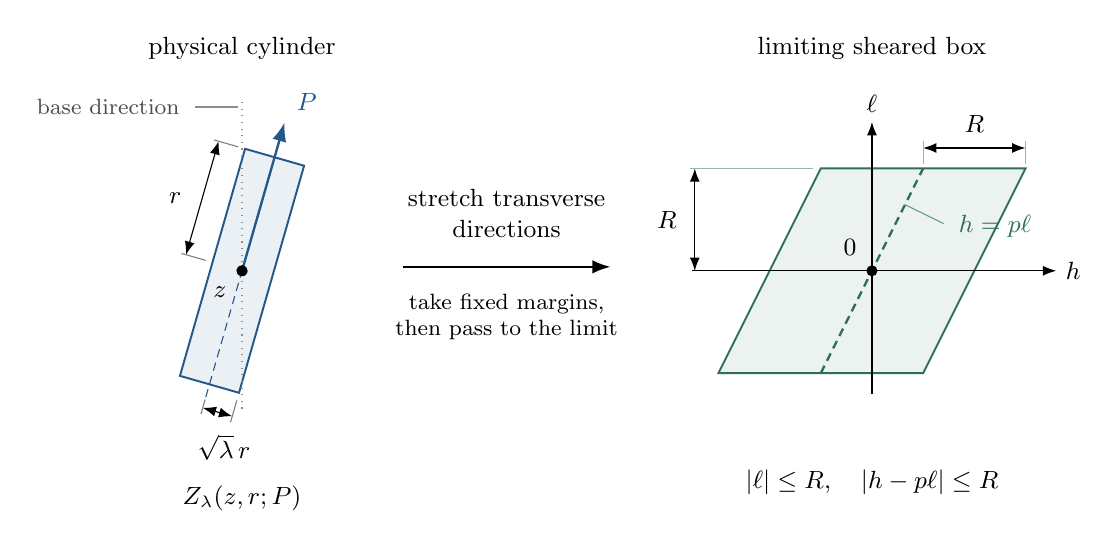
\begin{tikzpicture}[x=1cm,y=1cm,>=Latex,font=\small]
  \definecolor{fitblue}{RGB}{35,88,136}
  \definecolor{fitgreen}{RGB}{46,112,85}
  \node at (2.25,4.68) {physical cylinder};
  \node at (10.25,4.68) {limiting sheared box};
  \node[anchor=north,align=center] at (2.25,-0.76)
      {$Z_\lambda(z,r;P)$};
  \begin{scope}[shift={(2.25,1.85)},rotate=-16]
    \filldraw[draw=fitblue,fill=fitblue!9,line width=0.7pt]
        (-0.39,-1.50) rectangle (0.39,1.50);
    \draw[fitblue,densely dashed] (0,-1.67)--(0,0);
    \draw[fitblue,->,line width=0.85pt] (0,0)--(0,1.96)
        node[above right=1pt] {$P$};
    \fill (0,0) circle (2pt);
    \node[below left=3pt] at (0,0) {$z$};
    \draw[<->] (-0.74,0)--(-0.74,1.50)
        node[midway,left=4pt] {$r$};
    \draw[black!50] (-0.80,0)--(-0.48,0)
                        (-0.80,1.50)--(-0.48,1.50);
    \draw[<->] (0,-1.81)--(0.39,-1.81);
    \draw[black!50] (0,-1.70)--(0,-1.89)
                        (0.39,-1.60)--(0.39,-1.89);
    \node[below=4pt] at (0.28,-1.81) {$\sqrt\lambda\,r$};
  \end{scope}
  \draw[black!45,dotted] (2.25,0.10)--(2.25,4.05);
  \fill (2.25,1.85) circle (2pt);
  \node[anchor=east,font=\footnotesize,black!70] at (1.58,3.93)
      {base direction};
  \draw[black!45] (1.65,3.93)--(2.20,3.93);
  \draw[->,line width=0.8pt] (4.30,1.90)--(6.93,1.90);
  \node[align=center] at (5.61,2.58)
      {stretch transverse\\directions};
  \node[align=center,font=\footnotesize] at (5.61,1.26)
      {take fixed margins,\\then pass to the limit};
  \begin{scope}[shift={(10.25,1.85)}]
    \filldraw[draw=fitgreen,fill=fitgreen!9,line width=0.7pt]
        (-1.95,-1.30)--(0.65,-1.30)--(1.95,1.30)--(-0.65,1.30)--cycle;
    \draw[->] (-2.28,0)--(2.34,0) node[right] {$h$};
    \draw[->] (0,-1.57)--(0,1.89) node[above] {$\ell$};
    \draw[fitgreen,densely dashed,line width=0.85pt]
        (-0.65,-1.30)--(0.65,1.30);
    \node[fitgreen,anchor=west] at (0.98,0.57) {$h=p\ell$};
    \draw[fitgreen!70] (0.91,0.60)--(0.42,0.84);
    \fill (0,0) circle (2pt);
    \node[above left=3pt] at (0,0) {$0$};
    \draw[<->] (0.65,1.56)--(1.95,1.56)
        node[midway,above=2pt] {$R$};
    \draw[fitgreen!50] (0.65,1.35)--(0.65,1.65)
                          (1.95,1.35)--(1.95,1.65);
    \draw[<->] (-2.25,0)--(-2.25,1.30)
        node[midway,left=3pt] {$R$};
    \draw[fitgreen!50] (-2.31,1.30)--(-0.75,1.30);
    \node[align=center] at (0,-2.69)
        {$|\ell|\le R,\quad |h-p\ell|\le R$};
  \end{scope}
\end{tikzpicture}
\caption{From thin cylinders to sheared fitting domains. The left panel
 shows a two-dimensional section of $Z_\lambda(z,r;P)$, with axial radius
 $r$ and transverse radius $\sqrt\lambda\,r$; the dotted line indicates the
 base direction used for rescaling. Stretching transverse directions makes
 the small inclination of a nearby fitted axis visible as a finite shear.
 Fixed margins give contained sheared boxes, and passage to the limit
 yields $Q_R(z;p)$, shown on the right in increment coordinates $(h,\ell)$.
 The panels are schematic: the finite-scale cylinder image is not asserted
 to equal the limiting box.}
\label{fig:anisotropic-fit}
\end{figure}


This proves equicontinuity on compact sets. Given an accuracy $\varepsilon>0$, first fix $S>0$ so small that $2\Lambda S<\varepsilon/3$. For a fixed box, \eqref{eq:normalized-fit-slopes} now bounds its coefficients by some finite $C_{K,S}$. Choose the increments sufficiently small, depending on this bound and $S$, that \eqref{eq:normalized-fit-domain} holds and the affine increment in \eqref{eq:normalized-fit} is less than $\varepsilon/3$. For all sufficiently large $i$, \eqref{eq:base-norm-bounds} and \eqref{eq:normalized-fit} then bound the value increment by $2\varepsilon/3$. Discard an initial segment so that all domains contain the compact box. The threshold in $i$ may depend on $\varepsilon$; the finitely many remaining preceding continuous functions can be included by decreasing the increment size. The local bounds and domain exhaustion now give a locally uniformly convergent subsequence, with limit $v$ and $v(0,0)=0$.

The jet operators $X[(p_x,1+\lambda_i p_t)]$ converge locally uniformly to $X[(p_x,1)]$. Viscosity stability gives \eqref{eq:limit-pde}; equivalently, strictify a smooth upper or lower test for $v$, choose nearby touching points for $v_i$, and pass to the limit in \eqref{eq:rescaled-pde}. To pass the fits, fix a center and a target radius $R>0$, and take $S=4R$ in \eqref{eq:normalized-fit}. After a further subsequence its bounded coefficients converge to $p,q$. The shears $p_i'/(1+\lambda_i q_i')$ converge to $p$. Every increment with $|\ell|\le R$ and $|h-p\ell|\le R$ then satisfies \eqref{eq:normalized-fit-domain}, uniformly, for all sufficiently large $i$. Passing to the limit in \eqref{eq:normalized-fit} yields \eqref{eq:limit-fit} with
\[
  a=q+|p|^2/2,\qquad C_0=8\Lambda=256.
\]
The additional subsequence may depend on the chosen center and radius: the limit function $v$ stays fixed, and \eqref{eq:limit-fit} asserts existence separately for each choice.

Finally suppose that $v$ is affine. Since $v(0,0)=0$, write $v(x,t)=p\cdot x+qt$. In the physical coordinates consider
\[
  \widetilde P_i=c_i(\sqrt{\lambda_i}p,1+\lambda_i q).
\]
These slopes are nonzero for large $i$. The cylinders $Z_{\lambda_i}(z_i,r_i;\widetilde P_i)$ lie in one fixed box of the rescaled coordinates. In fact, if
\[
  N_i=\bigl(\lambda_i|p|^2+(1+\lambda_i q)^2\bigr)^{1/2}\longrightarrow1,
\]
a point in such a cylinder, in units of $r_i$, is $s(\sqrt{\lambda_i}p,1+\lambda_i q)/N_i+\sqrt{\lambda_i}\xi$ with $|s|\le1$, $|\xi|\le1$, and $\xi$ perpendicular to the axis. Its rescaled coordinates satisfy $|x|\le |p|/N_i+1$ and $|t|\le1+\sqrt{\lambda_i}$. On this fixed box the residual for the proposed fit is exactly
\[
  r_i c_i\lambda_i\bigl(v_i(x,t)-p\cdot x-qt\bigr)=o(\lambda_i r_i)
\]
uniformly, by local uniform convergence and the upper bound for $c_i$. It is eventually at most $\lambda_i r_i$ on the whole cylinder. This makes $\lambda_i$ good for $U_i$ at $(z_i,r_i)$, contrary to Lemma~\ref{lem:bad-scales}. Hence $v$ is nonaffine.
\end{proof}

\begin{proof}[Proof of Proposition~\ref{prop:power-decay}]
If no power bound held, Lemma~\ref{lem:bad-scales} and Proposition~\ref{prop:nonaffine-limit} would produce a nonaffine entire solution satisfying all hypotheses of Theorem~\ref{thm:liouville}, with $m=d$ and $C_0=256$. The theorem makes that solution affine, a contradiction. Hence a power bound holds. Reducing its exponent if necessary gives $\gamma\le1$. Since the family $\mathcal U$ and the function $b$ were fixed solely by $d$, the constants in \eqref{eq:power-decay} depend only on $d$.
\end{proof}

\subsection{From cylinder fits to a H\"older gradient}

We finish the reduction by extracting the uniform estimate from \eqref{eq:power-decay}. The exponent comes from the inscribed balls: their radii are $\sqrt\lambda r$, whereas the fitting error is $\lambda r$.

\begin{proof}[Proof of Theorem~\ref{thm:main}, assuming Theorem~\ref{thm:liouville}]
Take $B,\gamma,s_0$ from Proposition~\ref{prop:power-decay}. At every center $z\in\overline B_{1/2}^n$ one has $D(z)\ge d_0:=1/4$. Choose $A_0>Bd_0^{-\gamma}$. There is $r_0>0$, depending only on $d$, such that for all $0<r\le r_0$,
\[
  r/d_0\le\min\{s_0,1/8\},\qquad A_0r^\gamma<1.
\]
For every $U\in\mathcal U$ and each such center and radius,
\[
  \beta_U(z,r)\le b(r/D(z))
       \le B(r/d_0)^\gamma<A_0r^\gamma.
\]
Thus $\lambda=A_0r^\gamma$ is good, with the same constants for all functions and centers.

Fix $U\in\mathcal U$. Set
\[
  r_j=2^{-j}r_0,\qquad
  \rho_j=\sqrt{A_0}\,r_j^{1+\gamma/2},\qquad j\ge0,
\]
and at each center $z\in\overline B_{1/2}^n$ choose a fitted slope $P_j(z)$ for the parameter $A_0r_j^\gamma$. The fit holds on the inscribed ball $\overline B_{\rho_j}(z)$, with error at most $A_0r_j^{1+\gamma}$. Comparing consecutive fits on their common ball $\overline B_{\rho_{j+1}}(z)$ gives
\[
  |P_j(z)-P_{j+1}(z)|
   \le\frac{A_0(r_j^{1+\gamma}+r_{j+1}^{1+\gamma})}{\rho_{j+1}}
   \le C r_j^{\gamma/2}.
\]
The geometric tail converges uniformly in $U$ and $z$. Consequently there is a vector $P_\infty(z)$ with
\begin{equation}\label{eq:slope-tail}
  |P_j(z)-P_\infty(z)|\le C r_j^{\gamma/2}.
\end{equation}
If $0<|h|\le\rho_0$, choose $j$ so that $\rho_{j+1}<|h|\le\rho_j$. The fit at radius $r_j$ and \eqref{eq:slope-tail} give
\begin{align*}
  \frac{|U(z+h)-U(z)-P_\infty(z)\cdot h|}{|h|}
   &\le\frac{A_0r_j^{1+\gamma}}{\rho_{j+1}}
            +|P_j(z)-P_\infty(z)|\\
   &\le C r_j^{\gamma/2}\le C'|h|^{\alpha_d},
\end{align*}
where
\begin{equation}\label{eq:holder-exponent}
  \alpha_d=\frac{\gamma}{2+\gamma}\in(0,1/3].
\end{equation}
The final inequality follows from
$\rho_{j+1}=\sqrt{A_0}\,2^{-(1+\gamma/2)}r_j^{1+\gamma/2}$ and
$(1+\gamma/2)\alpha_d=\gamma/2$. Thus $U$ is differentiable at every such $z$, with gradient $P_\infty(z)$, and
\begin{equation}\label{eq:uniform-taylor-estimate}
  |U(z+h)-U(z)-\nabla U(z)\cdot h|
       \le C|h|^{1+\alpha_d}\qquad(|h|\le\rho_0).
\end{equation}
All increments here remain in $G$, since each lies in one of the admissible inscribed balls. The original Lipschitz bound gives $|\nabla U(z)|\le L$.

To compare gradients, take $z,z'\in\overline B_{1/2}^n$ with $\ell=|z-z'|\le\rho_0/2$ and $\ell>0$, and fix any unit vector $e\in\R^n$. The evaluation point $z'+\ell e$ need not lie in $B_{1/2}^n$; the Taylor estimates centered at $z$ and $z'$ still apply. Applying \eqref{eq:uniform-taylor-estimate} at $z'$ to the increment $\ell e$ gives
\[
  U(z'+\ell e)-U(z')
       =\ell\nabla U(z')\cdot e+O(\ell^{1+\alpha_d}).
\]
Applying the same estimate at $z$ to the increments $z'-z$ and $z'+\ell e-z$, whose lengths are at most $2\ell$, gives
\[
  U(z'+\ell e)-U(z')
       =\ell\nabla U(z)\cdot e+O(\ell^{1+\alpha_d}).
\]
The constants are independent of $e,U,z,z'$. Subtracting and taking the supremum over unit vectors proves
\[
  |\nabla U(z)-\nabla U(z')|\le C\ell^{\alpha_d}.
\]
For larger distances the same estimate follows, after increasing $C$, from $|\nabla U|\le L$. Restriction to points $(y,0)$ therefore gives the claimed uniform gradient norm and H\"older seminorm for every normalized $u$.

Finally, if $u$ is as in Theorem~\ref{thm:main} and its oscillation is $M>0$, then $(u-u(0))/M$ is a normalized solution: positive scaling and addition of constants preserve the viscosity equation by transformation of tests. Multiplying the normalized estimates by $M$ gives the theorem. If $M=0$, the function is constant and the conclusion is immediate.
\end{proof}

It remains to prove Theorem~\ref{thm:liouville}. The following sections use only its equation and fitting hypothesis; the original infinity-harmonic family will no longer enter the argument.

\section{Compactness and quadratic envelopes}\label{sec:limiting-tools}

We begin the proof of Theorem~\ref{thm:liouville}. Write
$\Aclass_{m,C_0}$ for the class of continuous functions on
$\R^m\times\R$ that solve \eqref{eq:limit-pde} and have the fits
\eqref{eq:limit-fit} at every center and radius. We may enlarge $C_0$ to
$\max\{C_0,1\}$. Constants denoted by $C$ in estimates for this class
may depend on $m$ and $C_0$.

\subsection{Changes of frame and compactness}

\begin{lemma}[Changes of frame]\label{lem:frame-invariance}
Let $v\in\Aclass_{m,C_0}$, $z_0=(x_0,t_0)$, $R>0$, and
$(p_0,a_0)\in\R^m\times\R$. Then
\begin{equation}\label{eq:frame-change}
  \bar v(y,s)=
  \frac{v(x_0+R(y+p_0s),t_0+Rs)-v(x_0,t_0)}{R}
       -p_0\cdot y-\left(a_0+\frac{|p_0|^2}{2}\right)s
\end{equation}
belongs to $\Aclass_{m,C_0}$. A fit $(p,a)$ for $v$ at the
corresponding center and radius $R\rho$ becomes the fit
$(p-p_0,a-a_0)$ for $\bar v$ at radius $\rho$.
\end{lemma}

\begin{proof}
Set
\[
  B=\begin{pmatrix}I_m&p_0\\0&1\end{pmatrix}.
\]
For smooth functions, at corresponding points,
$\nabla_y\bar v=\nabla_xv-p_0$ and
$D^2\bar v=R B^{\mathsf T}D^2vB$. Since
$B(\nabla_y\bar v,1)=(\nabla_xv,1)$, this gives
$F[\bar v]=R F[v]$. Pulling back an upper or lower smooth test gives
the same implication in the viscosity sense. For the fits, an
increment $(h,\ell)$ in the new variables corresponds to
$R(h+p_0\ell,\ell)$. The old affine increment, divided by $R$ and
with the affine part of \eqref{eq:frame-change} subtracted, is
\[
  (p-p_0)\cdot h+
  \left(a-a_0-\frac{|p-p_0|^2}{2}\right)\ell.
\]
The old box conditions become
$|\ell|\le\rho$ and $|h-(p-p_0)\ell|\le\rho$, and the error is
$C_0\rho$.
\end{proof}

We say that $v$ is \emph{centered at $z_c$} if $v(z_c)=0$ and
$(0,0)$ is a fit there of radius $1$. Choosing $(p_0,a_0)$ to be a
fit at $(z_0,R)$ in \eqref{eq:frame-change} produces a function
centered at the origin. We will also center at $(0,1)$, using a
translation of the time coordinate. Put
\[
  L(K)=1+\log K\qquad(K\ge2),\qquad
  \mathcal B_K=\{(x,t):|x|\le K,\ |t|\le K\}.
\]

Comparisons of fits across scales give the logarithmic parameter bounds
below. They yield compactness after centering and uniform subquadratic
spatial growth, which will confine the quadratic-envelope optimizers.
The estimates use only the fits; the equation enters when the limit is
identified.

\begin{lemma}[Bounds and compactness from fits]\label{lem:fit-compactness}
Suppose that $v\in\Aclass_{m,C_0}$ is centered at either $(0,0)$ or
$(0,1)$. For $K\ge2$ one has
\begin{equation}\label{eq:centered-growth}
  |v(x,t)|\le C K L(K)^2\qquad ((x,t)\in\mathcal B_K).
\end{equation}
Every fit $(p,a)$ at a center in $\mathcal B_K$, of any radius $r>0$,
satisfies
\begin{equation}\label{eq:fit-parameter-bound}
  |p|+|a|\le C\bigl(L(K)+|\log r|\bigr).
\end{equation}
In particular, for a center $(x,t)\in\mathcal B_K$,
\begin{align}
  |v(x+h,t)-v(x,t)|
    &\le Cr\bigl(L(K)+|\log r|\bigr)
       &&(|h|\le r),\label{eq:spatial-fit-modulus}\\
  |v(x,t+\tau)-v(x,t)|
    &\le C|\tau|\bigl(L(K)+|\log|\tau||\bigr)^2
       &&(0<|\tau|\le\tfrac12).\label{eq:time-fit-modulus}
\end{align}
For either fixed choice of center, every sequence of centered
members has a locally uniformly convergent subsequence, and its
limit belongs to $\Aclass_{m,C_0}$ and is centered at that same
point. Moreover, on every compact time interval these members have
uniformly subquadratic growth in $x$:
\begin{equation}\label{eq:uniform-subquadratic-growth}
  \lim_{M\to\infty}\ 
  \sup_{\substack{v\text{ centered}\\ |x|\ge M,\ t\in J}}
       \frac{|v(x,t)|}{|x|^2}=0
  \qquad(J\Subset\R).
\end{equation}
\end{lemma}

\begin{proof}
We prove the estimates for centering at the origin. Translation by
one unit in time gives the other case after enlarging the boxes by a
fixed factor.

First compare two fits $(p,a),(p',a')$ at the same center, with
radii $R$ and $R'\in[R,2R]$. On the horizontal slice $\ell=0$,
both estimates hold for $|h|\le R$, so
$|p-p'|\le 3C_0\le4C_0$. Write
\[
  \ell_{p,a}(h,\ell)=p\cdot h+
                \left(a-\frac{|p|^2}{2}\right)\ell.
\]
With $c=(2+8C_0)^{-1}$, the point $(p cR,cR)$ lies in both sheared
boxes. At this point
\[
  (\ell_{p,a}-\ell_{p',a'})(p cR,cR)
    =\left(a-a'+\frac{|p-p'|^2}{2}\right)cR.
\]
The two fitting errors sum to at most $3C_0R$. It follows that
$|a-a'|\le 3C_0/c+8C_0^2$. Thus the differences of both parameters
are bounded by one constant whenever the radii differ by at most a
factor of two. Comparing along successive dyadic radii with the
centered fit of radius $1$ gives, for every fit at the origin of
radius $r$,
\begin{equation}\label{eq:origin-fit-bound}
  |p|+|a|\le C(1+|\log r|).
\end{equation}

Fix $K\ge2$. Choose once and for all a sufficiently large constant
$A=A(m,C_0)$ and set
$R=A K L(K)$. If $(p_R,a_R)$ is any fit of radius $R$ at the
origin, then $\mathcal B_K$ lies in its sheared box with
\[
  |t|\le R/4,\qquad |x-p_Rt|\le R/4.
\]
Indeed, \eqref{eq:origin-fit-bound} bounds the latter offset by
$K(1+C(1+\log R))$, while
$\log R\le\log A+2L(K)$. Since $L(K)\ge1$, the asserted two
inequalities hold for all $K\ge2$ once $A$ is chosen larger than a
fixed multiple of $1+\log A$. Such a choice is possible because
$\log A/A\to0$. The fit at radius $R$ now gives
\[
  |v(x,t)|
  \le C_0R+|p_R|K+
      \left(|a_R|+\frac{|p_R|^2}{2}\right)K
  \le C K L(K)^2,
\]
which is \eqref{eq:centered-growth}.

Let $z=(x,t)\in\mathcal B_K$, and compare a fit $(p_z,a_z)$ of
radius $R$ at $z$ with the enclosing fit $(p_R,a_R)$. For
horizontal increments of length at most $R/2$ from $z$, the
enclosing estimate can be subtracted at the two endpoints, with
error at most $2C_0R$. Comparison with the fit at $z$ therefore
gives $|p_z-p_R|\le6C_0$. Set
$c'=(4(1+6C_0))^{-1}$. The increments
$(p_z c'R,c'R)$ from $z$ remain in both boxes: in the enclosing
box the transverse offset is at most
$R/4+6C_0c'R\le R/2$, and the time offset is at most $R/2$.
The same affine-increment identity used above gives a bound on
$|a_z-a_R|$ depending only on $C_0$. Hence
$|p_z|+|a_z|\le C L(K)$. Dyadic comparisons at $z$, from radius
$R$ to an arbitrary radius $r$, give
\[
  |p|+|a|
  \le C L(K)+C(1+|\log(r/R)|)
  \le C\bigl(L(K)+|\log r|\bigr),
\]
as claimed. These comparisons apply to every choice of fit.

Using a fit of radius $r$ on the horizontal slice proves
\eqref{eq:spatial-fit-modulus}. For a time increment $\tau$ with
$0<|\tau|\le1/2$, put
$B=L(K)+|\log|\tau||$ and choose the fit radius
$r=A'|\tau|B$. Here $A'$ is a constant to be fixed, independent of
$K$ and $\tau$. Since $B\ge1$,
\[
  |\log r|\le|\log|\tau||+\log A'+\log B
       \le2B+\log A'.
\]
The fit-parameter bound consequently gives
$|p|\le C(3+\log A')B$. Choose $A'\ge1$ sufficiently large that
$A'\ge C(3+\log A')$. This choice is possible and is made before
$K$ and $\tau$ vary. Then $|\tau|\le r$ and $|p\tau|\le r$, so
the vertical increment lies in the fitted box. In that estimate,
the affine time coefficient and error are bounded by
\[
  \left(|a|+\frac{|p|^2}{2}\right)|\tau|+C_0r
      \le C|\tau|B^2.
\]
This proves \eqref{eq:time-fit-modulus}.

The two moduli, applied successively to a spatial and a time
increment in a slightly larger box, give equicontinuity on compact
sets. The growth bound gives local uniform boundedness.
Arzel\`a--Ascoli and a diagonal choice of subsequence therefore
give local uniform convergence. To pass an upper viscosity test
to the limit, add a positive fourth-order term at its contact,
preserving its first and second derivatives and making the
contact strict on a small closed ball. Maxima of the sequence
minus this modified test on that ball converge to the contact,
so they are interior for large indices. The viscosity
inequalities there pass to the limit by continuity of $F$.
Subtracting the fourth-order term and using minima treats a
lower test. To pass the fits, fix one
center and one radius $r$. By \eqref{eq:fit-parameter-bound}, pass
to a further subsequence of the corresponding fits with
$(p_j,a_j)\to(p,a)$. For a point with
$|\ell|\le r$ and $|h-p\ell|\le r$, use in the $j$th fitted box
the increment
$h_j=p_j\ell+(h-p\ell)$. It converges to $h$ and belongs to that
closed box. Local uniform convergence gives the limiting
inequality. This subsequence may depend on the fixed center and
radius, which is sufficient for existence of a fit at each such
pair. The centered fit passes directly to the limit.
Finally, for $t$ in a fixed compact interval,
\eqref{eq:centered-growth} gives a bound of the form
$C_J(1+|x|)(1+\log(2+|x|))^2$, uniformly in the centered class.
Dividing by $|x|^2$ proves
\eqref{eq:uniform-subquadratic-growth}.
\end{proof}

If a family instead has one common prescribed value and one common
fit at a fixed center and radius, one fixed change of frame
\eqref{eq:frame-change} reduces it to the centered case. The
corresponding local bounds and compactness hold with constants
also depending on those prescribed data.

\subsection{Quadratic envelopes and their slopes}

Let $I\subseteq\R$ be an open interval. We say that a continuous
function $f$ on $\R^m\times I$ has \emph{subquadratic spatial
growth on compact time intervals} if, for every $J\Subset I$,
\[
  \lim_{M\to\infty}
  \sup_{\substack{|x|\ge M\\t\in J}}\frac{|f(x,t)|}{|x|^2}=0.
\]
For $\ell>0$, with the indicated time argument in $I$, define
\begin{equation}\label{eq:envelope-definitions}
  \begin{split}
  \Penv_\ell f(x,t)
    &=\sup_y\left\{f(y,t+\ell)-\frac{|y-x|^2}{2\ell}\right\},\\
  \Menv_\ell f(x,t)
    &=\inf_y\left\{f(y,t-\ell)+\frac{|y-x|^2}{2\ell}\right\}.
  \end{split}
\end{equation}
Set $\Penv_0f=\Menv_0f=f$. The following quadratic slice
comparisons are useful for the limiting equation; compare
\cite[Section~3]{EvansSavin2008}. Convexity of Hamilton--Jacobi envelopes also
appears in the comparison theory of Armstrong, Crandall, Julin, and Smart
\cite[Proposition~2.3]{ArmstrongCrandallJulinSmart2011}. Their Hamiltonian
hypotheses do not cover the limiting equation here; we prove the required
properties directly.
For a fixed center, convexity in the length will give monotone envelope
slopes. The moving-center form records the cost of shifting the center;
its midpoint inequality will control velocity differences in
Section~\ref{sec:discrete-propagation}.

\begin{lemma}[Quadratic envelopes]\label{lem:quadratic-envelopes}
Suppose that $f$ has the preceding growth property. The extrema
in \eqref{eq:envelope-definitions} are attained. The envelopes
are continuous jointly in their center and length, including
length zero wherever the time arguments remain in $I$. Whenever
the expressions are defined,
\begin{equation}\label{eq:envelope-composition}
  \Penv_\ell(\Penv_hf)=\Penv_{\ell+h}f,\qquad
  \Menv_\ell(\Menv_hf)=\Menv_{\ell+h}f.
\end{equation}
If $f$ is a viscosity subsolution of \eqref{eq:limit-pde}, then,
for every affine path $x(\ell)=x_0+d\ell$ and every fixed $t$,
\begin{equation}\label{eq:path-envelope-convexity}
  \ell\longmapsto
  \Penv_\ell f(x(\ell),t)+|d|^2\ell\log\ell
  \quad\text{is convex}
\end{equation}
on its allowed range $\ell\ge0$, with $\ell\log\ell=0$ at zero.
In particular $\ell\mapsto\Penv_\ell f(x,t)$ is convex.
If $f$ is a viscosity supersolution, then
$\ell\mapsto\Menv_\ell f(x,t)$ is concave.
If $f_j\in C(\R^m\times I)$, $f_j\to f$ locally uniformly, and
\[
  \lim_{M\to\infty}\sup_j\sup_{\substack{|y|\ge M\\t\in J}}
      \frac{|f_j(y,t)|}{|y|^2}=0\qquad(J\Subset I),
\]
then
$\Penv_\ell f_j\to\Penv_\ell f$ and $\Menv_\ell f_j\to\Menv_\ell f$
locally uniformly in the allowed centers and positive lengths.
\end{lemma}

\begin{proof}
Fix a compact range of centers and of allowed positive lengths.
Uniform subquadratic growth and the quadratic cost force all
maximizers and minimizers into a common bounded spatial set.
They exist there, and the maximum and minimum of a continuous
function over this fixed compact set depend continuously on the
parameters. The same bounded-set conclusion holds when the
length varies in $(0,\ell_0]$. On that set the values of $f$ are
bounded. Comparison with the competitor $y=x$ then gives
$|y-x|^2\le C\ell$ for an optimizer as $\ell\downarrow0$.
Uniform continuity of $f$ on the compact set gives convergence
to $f(x,t)$ locally uniformly, as well as $y\to x$ locally
uniformly. This proves continuity at zero. The composition
identities follow by optimizing first over the intermediate
point and using
\[
  \inf_y\left\{\frac{|y-x|^2}{2\ell}
           +\frac{|z-y|^2}{2h}\right\}
       =\frac{|z-x|^2}{2(\ell+h)}.
\]

For the convexity assertion, let
$g(\ell)=\Penv_\ell f(x(\ell),t)$, and let a smooth function
$\psi$ touch $g$ from above at $\ell_0>0$. Choose an optimizer
$y_0$ at that length. After a constant adjustment,
\[
  \Psi(y,\ell)=\psi(\ell)+\frac{|y-x(\ell)|^2}{2\ell}
\]
touches $(y,\ell)\mapsto f(y,t+\ell)$ from above at
$(y_0,\ell_0)$. Put $q=(y_0-x(\ell_0))/\ell_0$, which is the
horizontal gradient of $\Psi$ there. Along the direction
$(q,1)$, the Hessian of the quadratic term has value
$|d|^2/\ell_0$. For example, writing $r=y-x(\ell)$, its value
along a direction with $r$-velocity $q-d$ is
$\ell_0^{-1}|q-d-r/\ell_0|^2=|d|^2/\ell_0$.
The viscosity inequality gives
$\psi''(\ell_0)+|d|^2/\ell_0\ge0$. Thus every upper test for
$g(\ell)+|d|^2\ell\log\ell$ has nonnegative second derivative
at positive lengths. This is the one-dimensional viscosity
criterion for convexity. To see it directly, a failure of
convexity on $[a,b]$ lets one place a strictly concave quadratic
above the chord but below the function somewhere; the positive
maximum of their difference yields an upper test with negative
second derivative. Continuity at zero extends the convexity to
that endpoint.

Finally, the map $\widetilde f(x,t)=-f(x,-t)$ exchanges
subsolutions and supersolutions of \eqref{eq:limit-pde}, as
pullback reverses the sign of $F$. It also gives
$\Penv_\ell\widetilde f(x,t)=-\Menv_\ell f(x,-t)$.
The assertion for $\Menv$ follows.

For the last convergence assertion, fix a compact range of allowed centers
and positive lengths. The common subquadratic bound and the local uniform
bounds confine every optimizer for $f_j$ and for $f$ to one compact spatial
set, by the first argument of the proof. On that set the functions inside
the supremum and infimum converge uniformly. Their extrema therefore
converge uniformly on the chosen parameter range.
\end{proof}

For a positive allowed length define the two slopes
\begin{equation}\label{eq:envelope-slopes}
  \Senv_\ell^+f(z)=\frac{\Penv_\ell f(z)-f(z)}{\ell},
  \qquad
  \Senv_\ell^-f(z)=\frac{f(z)-\Menv_\ell f(z)}{\ell}.
\end{equation}
For a smooth function, the quantity
$H_{\mathrm{sm}}=f_t+|\nabla_xf|^2/2$ satisfies
\[
  F[f]=(\partial_t+\nabla_xf\cdot\nabla_x)H_{\mathrm{sm}}.
\]
For the exact affine model
$f(x,t)=p\cdot x+(a-|p|^2/2)t+c$ in \eqref{eq:limit-fit}, one has
$H_{\mathrm{sm}}=a$, and direct optimization gives
\[
  \Penv_\ell f=f+a\ell,\qquad \Menv_\ell f=f-a\ell.
\]
The optimizing displacements are respectively $\ell p$ and $-\ell p$.
Thus both envelope slopes equal $a$, and both optimizer velocities,
directed toward increasing time, equal $p$. These identifications concern
the exact affine model; for a general fitted solution, $p,a$ remain the
parameters of the chosen fit. For a general smooth function, a first-order
expansion of the two quadratic optimizations formally gives
$\Senv_\ell^\pm f=H_{\mathrm{sm}}+o(1)$ as $\ell\downarrow0$.
For a smooth solution the identity for $F[f]$ transports this quantity along
the direction $(\nabla_xf,1)$; its value may depend on the integral curve.
The next lemma supplies the slope statements used for continuous solutions.

Evans and Savin \cite[Theorem~3.1]{EvansSavin2008} proved the corresponding
slope monotonicity and equality of the finite limits at a fixed center under
their local boundedness and Lipschitz assumptions. The following formulation
uses envelopes on the full spatial domain under subquadratic growth,
separates the subsolution and supersolution conclusions, and allows the common
limit to be $-\infty$.

\begin{lemma}[Envelope slopes]\label{lem:envelope-slopes}
For a subsolution $f$ as in Lemma~\ref{lem:quadratic-envelopes},
$\Senv_\ell^+f(z)$ is nondecreasing in $\ell$ and
\begin{equation}\label{eq:subsolution-slope-order}
  \limsup_{\ell\downarrow0}\Senv_\ell^-f(z)
       \le\lim_{\ell\downarrow0}\Senv_\ell^+f(z).
\end{equation}
The right side may equal $-\infty$. For a supersolution,
$\Senv_\ell^-f(z)$ is nondecreasing and
\[
  \limsup_{\ell\downarrow0}\Senv_\ell^+f(z)
       \le\lim_{\ell\downarrow0}\Senv_\ell^-f(z).
\]
Consequently, for a
solution both slopes are nondecreasing and
\begin{equation}\label{eq:hamiltonian}
  \lim_{\ell\downarrow0}\Senv_\ell^+f(z)
  =\lim_{\ell\downarrow0}\Senv_\ell^-f(z)
  =:H_f(z)\in[-\infty,\infty).
\end{equation}
The function $H_f$ is upper semicontinuous.
\end{lemma}

\begin{proof}
Convexity of $\Penv_\ell f(z)$, with value $f(z)$ at zero,
gives the first monotonicity. Let
$\widetilde z_\ell=(y_\ell,t-\ell)$ be a backward optimizing
point for $\Menv_\ell f(z)$. Using $z$ as a forward competitor
from $\widetilde z_\ell$ gives
\[
  \Senv_\ell^-f(z)\le\Senv_\ell^+f(\widetilde z_\ell).
\]
The optimizer localization at length zero in
Lemma~\ref{lem:quadratic-envelopes} shows
$\widetilde z_\ell\to z$. Fix a small $h>0$ whose forward time
argument is allowed near $z$. For all sufficiently small
$\ell<h$, monotonicity bounds the right side by
$\Senv_h^+f(\widetilde z_\ell)$. Continuity for fixed $h$ gives
an upper limit at most $\Senv_h^+f(z)$. Now let $h\downarrow0$
to obtain \eqref{eq:subsolution-slope-order}. This order of
limits also covers the value $-\infty$.

Apply this conclusion to $\widetilde f(x,t)=-f(x,-t)$ to obtain
the supersolution statements. For a solution both monotone
limits exist and the two inequalities identify them. Each is
bounded above by the finite slope at any fixed positive allowed
length, proving the range in \eqref{eq:hamiltonian}. Locally in
$z$, choose a common small range of lengths. The common limit is
the infimum of the continuous functions $\Senv_\ell^+f(z)$ over
that range, so it is upper semicontinuous.
\end{proof}

\begin{lemma}[Bounds for fitted solutions]\label{lem:fitted-envelope-bounds}
For a member $v\in\Aclass_{m,C_0}$ centered at $(0,0)$ or $(0,1)$, $K\ge2$,
$z\in\mathcal B_K$, and $0<\ell\le K$, one has
\begin{equation}\label{eq:envelope-slope-bound}
  \Senv_\ell^+v(z)\le C L(K)^4,\qquad
  \Senv_\ell^-v(z)\le C L(K)^4.
\end{equation}
Every optimizing displacement for $\Penv_Kv(z)$ or
$\Menv_Kv(z)$ has length at most $C K L(K)^2$.
\end{lemma}

\begin{proof}
By Lemma~\ref{lem:envelope-slopes}, it suffices to bound the two
slopes at length $K$. Suppose an optimizing displacement has
length $BK$ with $B\ge2$. Comparing its value with the
competitor having no displacement, and using
\eqref{eq:centered-growth} in a box of size $(B+2)K$, gives
\[
  \frac{B^2K}{2}
     \le C BK\bigl(L(K)+\log B\bigr)^2.
\]
This estimate holds for the supremum and for the infimum.
Consequently
$B\le C(L(K)+\log B)^2\le2C L(K)^2+2C(\log B)^2$.
Choose a fixed $B_0$ so large that
$2C(\log B)^2\le B/2$ for $B\ge B_0$. The last inequality
then yields $B\le4C L(K)^2$ for $B\ge B_0$, and the same type
of bound holds when $B<B_0$. This proves the displacement
claim. The optimizer and its time argument now lie in a box of
size $C K L(K)^2$. Applying \eqref{eq:centered-growth} there
and observing that $L(C K L(K)^2)\le C L(K)$ bounds the
absolute values of $v$ there by $C K L(K)^4$. Dropping the
nonpositive cost in the expressions for the two slopes gives
\eqref{eq:envelope-slope-bound}.
\end{proof}

The criterion for the final limit is proved in
Lemma~\ref{lem:slope-rigidity}: if $v\in\Aclass_{m,C_0}$ and there are
$(b,t_0)\in\R^m\times\R$ and $B\in\R$ such that
\[
  \Senv_\ell^+v(b,t_0)=\Senv_\ell^-v(b,t_0)=B
       \qquad\text{for every }\ell>0,
\]
then $v$ is affine. The remaining argument will construct such a limit while
retaining an obstruction to affinity.

\section{An extremal horizontal defect and contact}\label{sec:envelope-contact}

We next turn a nonaffine member of $\Aclass_{m,C_0}$ into a
contact between a solution and a subsolution. A finite horizontal
probability configuration consists of positions
$y_1,\ldots,y_N\in\R^m$ and weights
$\theta_i>0$ with $\sum_i\theta_i=1$. Its mean and root mean
square radius are
\[
  x=\sum_i\theta_i y_i,\qquad
  r=\left(\sum_i\theta_i|y_i-x|^2\right)^{1/2}.
\]

\subsection{The barycentric envelope}

Let $I\subseteq\R$ be an open interval. For a continuous function $f$ on
$\R^m\times I$ with subquadratic spatial growth on compact time intervals,
define, for $s>0$,
\begin{equation}\label{eq:barycentric-envelope}
  \Cenv_s f(x,t)=
  \sup_{\substack{N,\ \theta_i>0,\ \sum_i\theta_i=1\\
                  \sum_i\theta_i y_i=x}}
   \left\{\sum_i\theta_i f(y_i,t)
             -\frac{\sum_i\theta_i|y_i-x|^2}{2s}\right\}.
\end{equation}
The supremum is over finite configurations, including the
single point $y_1=x$.
This operation averages one horizontal slice at the fixed time $t$;
$s$ controls the variance penalty. As the next lemma shows,
$\Cenv_s f(\cdot,t)-|\cdot|^2/(2s)$ is the least concave majorant of
$f(\cdot,t)-|\cdot|^2/(2s)$.

For the following estimate, suppose additionally that some $\kappa\ge0$
satisfies
\begin{equation}\label{eq:jensen-bound}
  \sum_i\theta_i f(y_i,t)-f(x,t)\le\kappa r
\end{equation}
for every $t\in I$ and every finite horizontal probability
configuration, with mean $x$ and radius $r$. Since
\[
  \kappa r-\frac{r^2}{2s}
   =\frac{\kappa^2s}{2}-\frac{(r-\kappa s)^2}{2s},
\]
the definition gives
\begin{equation}\label{eq:barycentric-sandwich}
  0\le\Cenv_s f(x,t)-f(x,t)
     \le\sup_{r\ge0}\left(\kappa r-\frac{r^2}{2s}\right)
     =\frac{\kappa^2s}{2}.
\end{equation}
The scalar maximum occurs at $r=\kappa s$. The extremal construction
below supplies a solution $v$ and a positive $\kappa$ attaining this bound.
We will prove that $\Cenv_t v-\kappa^2t/2$ is a subsolution for $t>0$;
the sandwich places it below $v$, with contact where equality holds and
a strictly positive unshifted gap.
The additional Jensen assumption applies only to this estimate; the next
lemma uses only the stated continuity and growth hypotheses.

\begin{lemma}[Barycentric envelope]\label{lem:barycentric-envelope}
Let $f$ have the preceding growth property on $\R^m\times I$.
For $s>0$ the supremum in \eqref{eq:barycentric-envelope} is
attained by a finite configuration, and
\begin{equation}\label{eq:barycentric-duality}
  \Cenv_s f(x,t)-\frac{|x|^2}{2s}
   =\min_{A\in\R^m}\ \max_{y\in\R^m}
       \left\{f(y,t)-\frac{|y|^2}{2s}-A\cdot(y-x)\right\}.
\end{equation}
Both extrema on the right are attained. Allowing any probability
measure of finite second moment and mean $x$ in
\eqref{eq:barycentric-envelope} gives the same value.
The function $\Cenv_s f(x,t)$ is continuous in $(x,t,s)$ for
$s>0$, and
\begin{equation}\label{eq:barycentric-semiconcavity}
  x\longmapsto\Cenv_s f(x,t)-\frac{|x|^2}{2s}
       \quad\text{is concave}.
\end{equation}
If $f_j\in C(\R^m\times I)$, $f_j\to f$ locally uniformly, and the sequence has the common
growth control
\[
  \lim_{M\to\infty}
  \sup_j\sup_{\substack{|y|\ge M\\t\in J}}
       \frac{|f_j(y,t)|}{|y|^2}=0
       \qquad(J\Subset I),
\]
then $\Cenv_s f_j\to\Cenv_s f$ locally uniformly for $s>0$.
\end{lemma}

\begin{proof}
For fixed $(t,s)$ put $g(y)=f(y,t)-|y|^2/(2s)$ and
\[
  \Gamma(A;x,t,s)=\sup_y\{g(y)-A\cdot(y-x)\}.
\]
The expression on the left of \eqref{eq:barycentric-duality}
is the supremum of $\sum_i\theta_i g(y_i)$ over configurations
of mean $x$, because
$\sum_i\theta_i|y_i-x|^2=\sum_i\theta_i|y_i|^2-|x|^2$.
It is therefore at most $\inf_A\Gamma(A;x,t,s)$.

Fix a compact range of $(x,t,s)$ with $s>0$. For $A\ne0$, use
$y=x-A/|A|$ in the supremum to get
$\Gamma(A;x,t,s)\ge |A|-C$ on this range. The value at $A=0$
is uniformly bounded above, since the negative quadratic part
of $g$ dominates the subquadratic growth of $f$. Thus every
minimizing sequence whose values are at most $\Gamma(0)+1$
lies in a fixed bounded set of slopes.
For slopes in that set, the quantity
$g(y)-A\cdot(y-x)$ tends uniformly to $-\infty$ as
$|y|\to\infty$. Its maximizing positions therefore lie in one
compact set. It follows that $\Gamma$ is continuous on the
relevant set, the minimum and maxima are attained, and their
value depends continuously on $(x,t,s)$.

Let $A_0$ be a minimizing slope, and let $E$ be its nonempty
compact set of maximizing positions. Then $x$ belongs to the
convex hull of $E$. Otherwise strict separation gives a vector
$e$ and $\delta>0$ with
$e\cdot(y-x)\ge\delta$ for all $y\in E$. If $y_h$ maximizes
$\Gamma(A_0+he;x,t,s)$ for $h>0$, the uniform compactness of
maximizers and continuity show that every limit of $y_h$ as
$h\downarrow0$ belongs to $E$. For small $h$,
$e\cdot(y_h-x)\ge\delta/2$, and hence
\[
  \Gamma(A_0+he;x,t,s)
   \le\Gamma(A_0;x,t,s)-h\delta/2,
\]
contradicting minimality. The finite-dimensional convex hull
theorem now represents $x$ as a convex combination of finitely
many points of $E$. Discard any zero weights. Their weighted
values of $g$ equal $\Gamma(A_0;x,t,s)$, proving the reverse
inequality in \eqref{eq:barycentric-duality} and finite
attainment in \eqref{eq:barycentric-envelope}.

The affine majorant
$g(y)\le\Gamma(A_0;x,t,s)+A_0\cdot(y-x)$ can also be
integrated against any probability measure of mean $x$ and
finite second moment. All terms are integrable by the growth
hypothesis. Thus such measures cannot increase the value.
The right side of \eqref{eq:barycentric-duality} is an infimum
of affine functions of $x$, so it is concave in $x$. This is
\eqref{eq:barycentric-semiconcavity}.

For the convergence assertion, on each compact range of
$(x,t,s)$ the same preceding bounds on slopes and maximizing
positions hold uniformly for $f_j$: local uniform convergence
gives common bounds near the compact range, and the common
subquadratic control handles large $y$. Both extrema in
\eqref{eq:barycentric-duality} can therefore be restricted to
fixed compact sets. On these sets the expressions converge
uniformly, proving the asserted local uniform convergence.
\end{proof}

\subsection{A common-time subsolution rule}

To test the barycentric envelope, we must combine subsolution inequalities
at several spatial points sharing one time variable. Lemma~\ref{lem:sum-rule} is
applied after separating and then synchronizing those times; the penalty
Hessian vanishes on the direction with time speed $1$ in every component,
which is the direction used by $F$.

\begin{lemma}[Common-time subsolutions]\label{lem:common-time-subsolution}
Let $v$ be a continuous viscosity subsolution of
\eqref{eq:limit-pde} on $\R^m\times I$, and fix positive weights
$\theta_i$ with $\sum_{i=1}^N\theta_i=1$. Define
\[
  V((y_i)_{i=1}^N,t)=\sum_{i=1}^N\theta_i v(y_i,t).
\]
If a $C^2$ function $\Phi$ touches $V$ from above at $(Y_0,t_0)$,
where $Y=(y_i)_{i=1}^N$, then
\begin{equation}\label{eq:common-time-inequality}
  D^2\Phi(Y_0,t_0)
   \left[\left(
       \bigl(\theta_i^{-1}\nabla_{y_i}\Phi(Y_0,t_0)\bigr)_{i=1}^N,
       1\right)\right]\ge0.
\end{equation}
\end{lemma}

\begin{proof}
Replace $\Phi$ by
$\Phi^\sharp=\Phi+|Y-Y_0|^4+|t-t_0|^4$. This makes the local
maximum strict while preserving the derivatives through order
two at the contact. Choose a small closed product neighborhood
of $((y_i^0,t_0))_{i=1}^N$, contained in the domain, such that
the diagonal points $(Y,t)$ lie in this strict neighborhood.
For independent time variables $T=(t_1,\ldots,t_N)$, put
\[
  \bar t=\frac1N\sum_i t_i,\qquad
  \chi(T)=\frac12\sum_i(t_i-\bar t)^2,\qquad
  \Psi_\lambda(Y,T)=\Phi^\sharp(Y,\bar t)+\lambda\chi(T).
\]
Maximize
$\sum_i\theta_i v(y_i,t_i)-\Psi_\lambda(Y,T)$ on the closed
product. Comparison with the original diagonal point and
boundedness on this product show
$\lambda\chi(T_\lambda)\le C$ at any maximum. Thus all
time deviations tend to zero as $\lambda\to\infty$. Every
limit of such maximum points is diagonal; dropping the
nonnegative penalty in the maximum inequality shows that its
diagonal limit is a maximum of $V-\Phi^\sharp$. Strictness
forces this limit to be $(Y_0,t_0)$. Hence all the maximum
points converge to the original point and are interior for
sufficiently large $\lambda$.

Fix one such $\lambda$ and one maximum. Set
\[
  q_i=\theta_i^{-1}\nabla_{y_i}
             \Phi^\sharp(Y_\lambda,\bar t_\lambda),
  \qquad
  \zeta_\lambda=((q_i,1))_{i=1}^N,\qquad
  A_\lambda=D^2\Psi_\lambda(Y_\lambda,T_\lambda),
\]
where $A_\lambda$ is written in the separate variables
$((y_i,t_i))_i$. Apply Lemma~\ref{lem:sum-rule} to the
functions $\theta_i v(y_i,t_i)$ and the test $\Psi_\lambda$.
For every $\eta>0$ it supplies closed superjets with Hessians
$X_i$ and first derivatives $D_{(y_i,t_i)}\Psi_\lambda$, with
$\operatorname{diag}(X_i)\le A_\lambda+\eta A_\lambda^2$.
Dividing each jet by the positive number $\theta_i$ gives a
closed superjet of $v$ with horizontal gradient $q_i$.
The viscosity inequalities therefore give
$X_i[(q_i,1)]\ge0$. Evaluating the matrix inequality on
$\zeta_\lambda$ yields
\[
  0\le\sum_iX_i[(q_i,1)]
     \le A_\lambda[\zeta_\lambda]
                   +\eta|A_\lambda\zeta_\lambda|^2.
\]
First let $\eta\downarrow0$, keeping $\lambda$ and its maximum
fixed. The quantities $A_\lambda$ and $\zeta_\lambda$ do not
depend on $\eta$, so $A_\lambda[\zeta_\lambda]\ge0$.
The time component of $\zeta_\lambda$ is $(1,\ldots,1)$,
which is in the kernel of $D^2\chi$. The linear map
$(Y,T)\mapsto(Y,\bar t)$ sends $\zeta_\lambda$ to
$((q_i)_i,1)$. We conclude that
\[
  D^2\Phi^\sharp(Y_\lambda,\bar t_\lambda)
       [((q_i)_i,1)]\ge0.
\]
Now let $\lambda\to\infty$. The maximum points converge to the
contact, and the horizontal derivatives converge there.
The derivatives of $\Phi^\sharp$ at that point are those of
$\Phi$, giving \eqref{eq:common-time-inequality}.
The time components of the first derivatives of
$\Psi_\lambda$ need no bound: they do not enter the direction
$(\nabla_xv,1)$ in the individual viscosity inequalities.
\end{proof}

\begin{corollary}[A barycentric subsolution]\label{cor:barycentric-subsolution}
Let $f\in C(\R^m\times(0,\infty))$ be a viscosity subsolution of
\eqref{eq:limit-pde} with subquadratic spatial growth on compact time
intervals. Then $(x,t)\mapsto\Cenv_t f(x,t)$ is a viscosity subsolution of
\eqref{eq:limit-pde} on $\R^m\times(0,\infty)$. For every $c\in\R$, the same
holds for $(x,t)\mapsto\Cenv_t f(x,t)-ct$.
\end{corollary}

\begin{proof}
Continuity follows from Lemma~\ref{lem:barycentric-envelope}. Fix $c\in\R$,
and let $\phi$ touch $(x,t)\mapsto\Cenv_t f(x,t)-ct$ from above at
$(x_0,t_0)$ with $t_0>0$. Choose an attaining finite configuration
$(\theta_i,y_i^0)$ for $\Cenv_{t_0}f(x_0,t_0)$, and keep its positive weights
fixed. For variable $Y=(y_i)_i$ let $X(Y)=\sum_i\theta_i y_i$ and define
\[
  \Phi(Y,t)=\phi(X(Y),t)+ct
              +\frac{\sum_i\theta_i|y_i-X(Y)|^2}{2t}.
\]
The defining supremum for $\Cenv_t$ shows that
$\sum_i\theta_i f(y_i,t)-\Phi(Y,t)$ has a local maximum at $(Y_0,t_0)$:
for nearby $(Y,t)$ it is at most
$\Cenv_t f(X(Y),t)-ct-\phi(X(Y),t)$, and equality holds at the chosen
configuration. Set $p=\nabla_x\phi(x_0,t_0)$. The individual horizontal
directions in Lemma~\ref{lem:common-time-subsolution} are
\[
  q_i=\theta_i^{-1}\nabla_{y_i}\Phi
       =p+\frac{y_i^0-x_0}{t_0}.
\]
Their weighted mean is $p$. Along the straight motion with velocities
$y_i'=q_i$ and $t'=1$, the mean has velocity $p$ and each offset $y_i-X$
has velocity $(y_i^0-x_0)/t_0$. Consequently, along this motion the variance
term is
\[
  \frac{\sum_i\theta_i
           |(y_i^0-x_0)(1+h/t_0)|^2}{2(t_0+h)}
    =\frac{t_0+h}{2t_0^2}
           \sum_i\theta_i|y_i^0-x_0|^2,
\]
which is affine in $h$. The term $ct$ is also affine, and the Hessian of the
remaining term along this motion is $D^2\phi[(p,1)]$.
Lemma~\ref{lem:common-time-subsolution}, applied to the subsolution
inequality for $f$, therefore gives $F[\phi](x_0,t_0)\ge0$. This proves the
claim for every $c$, including $c=0$.
\end{proof}

\subsection{Construction and slope of the contact}

\begin{proposition}[Extremal envelope contact]\label{prop:envelope-contact}
If $\Aclass_{m,C_0}$ contains a nonaffine member, then there
exist $\kappa\in(0,\infty)$ and $v\in\Aclass_{m,C_0}$ centered
at $z_*=(0,1)$ for which \eqref{eq:jensen-bound} holds with $f=v$ and
$I=\R$.
For $t>0$ set
\begin{equation}\label{eq:contact-envelope}
  W(x,t)=\Cenv_t v(x,t)-\frac{\kappa^2t}{2}.
\end{equation}
This function is continuous, has subquadratic spatial growth
on compact positive-time intervals, and is a viscosity
subsolution of \eqref{eq:limit-pde} on $\R^m\times(0,\infty)$.
It satisfies
\begin{equation}\label{eq:contact-sandwich}
  v(x,t)-\frac{\kappa^2t}{2}\le W(x,t)\le v(x,t)
       \quad(t>0),\qquad W(z_*)=v(z_*)=0,
\end{equation}
and $W(\cdot,t)-|x|^2/(2t)$ is concave for every $t>0$.
At every point of contact with $t>0$, the barycentric gap satisfies
\begin{equation}\label{eq:contact-barycentric-gap}
  W(x,t)=v(x,t)\quad\Longrightarrow\quad
  \frac{\Cenv_t v(x,t)-v(x,t)}{t}=\frac{\kappa^2}{2}>0.
\end{equation}
Finally,
\begin{equation}\label{eq:contact-slope}
  H_v(z_*)\in\R,\qquad
  \lim_{\ell\downarrow0}\Senv_\ell^+W(z_*)=H_v(z_*).
\end{equation}
\end{proposition}

\begin{proof}
\emph{A positive finite horizontal defect.}
Start with a nonaffine member $v^{(0)}$ and center it at the
origin using Lemma~\ref{lem:frame-invariance}. Some horizontal
slice of $v^{(0)}$ is nonaffine. To verify this, suppose instead
that
$v^{(0)}(x,t)=p(t)\cdot x+c(t)$ for every $t$. The coefficients
$p,c$ are continuous, as follows by evaluating the function at
$0$ and at the coordinate vectors. Direct optimization gives
\[
  \Penv_\ell v^{(0)}(x,t)
   =p(t+\ell)\cdot x+c(t+\ell)
                         +\frac{\ell}{2}|p(t+\ell)|^2.
\]
For every fixed $x,t$ this is convex in $\ell$. In each
convexity inequality, the coefficient of $x$ must vanish,
since the inequality holds for all $x\in\R^m$. Hence $p$
satisfies the affine interpolation identity on every interval,
and so is affine in $t$. On the other hand,
\eqref{eq:centered-growth}, applied at $x=\pm Ke$ and
$|t|\le K$, implies $|p(t)|\le C L(K)^2$. An affine function
of $t$ with this bound as $K\to\infty$ is constant. For
constant $p$, the displayed forward formula and its backward
counterpart
\[
  \Menv_\ell v^{(0)}(x,t)
   =p\cdot x+c(t-\ell)-\frac{\ell}{2}|p|^2
\]
show that $c$ is both convex and concave. It is therefore
affine, contradicting the choice of $v^{(0)}$.

A continuous nonaffine spatial slice has a nonzero midpoint
Jensen defect, since the midpoint identity everywhere would
make that slice affine. The transformation
$f(x,t)\mapsto-f(x,-t)$ preserves $\Aclass_{m,C_0}$: it
exchanges the two viscosity inequalities, and it sends a fit
$(p,a)$ to $(-p,a)$. It also changes the sign of a horizontal
Jensen defect. Apply this transformation if needed, so that
$v^{(0)}$ has a positive defect. Define
\begin{equation}\label{eq:jensen-supremum}
  \kappa=\sup_{\substack{t,\ \text{finite configurations}\\r>0}}
     \frac{\sum_i\theta_i v^{(0)}(y_i,t)-v^{(0)}(x,t)}{r}.
\end{equation}
Then $\kappa>0$. It is finite as well. For any configuration in
this supremum, choose a fit at its mean $(x,t)$ of radius $r$
and use \eqref{eq:frame-change} with these data. At time zero
the new positions are $(y_i-x)/r$, with mean zero and second
moment one. The defect divided by $r$ is unchanged, since the
affine terms cancel in the weighted difference. The new
function is centered. Its growth bound implies
$|\bar v(y,0)|\le C(1+|y|^2)$, with one constant for all these
normalizations. Integrating this inequality over a
configuration of second moment one bounds the quotient by a
fixed constant. Thus $0<\kappa<\infty$. More generally,
\eqref{eq:frame-change} preserves every such quotient, at
every time: spatial differences and their root mean square
radius both scale by $R$, and the subtracted affine terms
cancel.

\emph{Attainment after compactness.}
Choose configurations whose quotients in
\eqref{eq:jensen-supremum} tend to $\kappa$, and for each one
make the normalization just described. Denote the resulting
functions by $v_j$ and the normalized finite probability
measures by $\mu_j$. Then
\[
  v_j(0,0)=0,\qquad
  \int y\,d\mu_j=0,\qquad
  \int |y|^2\,d\mu_j=1,\qquad
  \int v_j(y,0)\,d\mu_j\longrightarrow\kappa.
\]
Every $v_j$ is centered at the origin, and every finite
configuration for it satisfies the Jensen bound with constant
$\kappa$. First use Lemma~\ref{lem:fit-compactness} to pass to
a locally uniform limit $\widehat v\in\Aclass_{m,C_0}$,
centered at the origin. The Jensen bound passes to this limit
for each fixed finite configuration.

The moment bound gives
$\mu_j(\{|y|>M\})\le M^{-2}$, so the measures are tight.
After a further subsequence they converge weakly to a
probability measure $\mu$. Lower semicontinuity of the second
moment gives $\int|y|^2\,d\mu\le1$. The mean remains zero:
the bound
$\int_{|y|>M}|y|\,d\mu_j\le M^{-1}$ makes the first moments
uniformly integrable, and the same bound holds for the limit.
To retain the extremal defect, we also need convergence of the value
integrals despite the varying functions and measures. For a compactly
supported continuous cutoff $\chi_M$, local uniform
convergence and weak convergence give
\[
  \int\chi_M(y)v_j(y,0)\,d\mu_j
       \longrightarrow
  \int\chi_M(y)\widehat v(y,0)\,d\mu.
\]
Choose $\chi_M=1$ on $\{|y|\le M\}$ and zero outside
$\{|y|<2M\}$. By
\eqref{eq:uniform-subquadratic-growth},
\[
  \int_{|y|>M}|v_j(y,0)|\,d\mu_j
  \le
  \sup_{\substack{j\\|y|>M}}\frac{|v_j(y,0)|}{|y|^2}
       \int|y|^2\,d\mu_j
  \longrightarrow0
\]
uniformly in $j$; the analogous tail bound holds for
$\widehat v$ and $\mu$. Letting first $j\to\infty$ and then
$M\to\infty$ proves
\begin{equation}\label{eq:extremal-measure}
  \int y\,d\mu=0,\qquad
  \int|y|^2\,d\mu\le1,\qquad
  \int\widehat v(y,0)\,d\mu-\widehat v(0,0)=\kappa.
\end{equation}

Apply \eqref{eq:barycentric-sandwich} to $\widehat v$. By
Lemma~\ref{lem:barycentric-envelope}, the measure in
\eqref{eq:extremal-measure} is admissible for the value of
$\Cenv_{1/\kappa}\widehat v(0,0)$. It gives
\[
  \Cenv_{1/\kappa}\widehat v(0,0)-\widehat v(0,0)
     \ge\kappa-\frac{\kappa}{2}\int|y|^2\,d\mu
     \ge\frac{\kappa}{2}.
\]
This is equality by \eqref{eq:barycentric-sandwich}. In
particular, loss of second moment in the weak limit causes no
loss of contact; the equality also forces
$\int|y|^2\,d\mu=1$.

Set $R=1/\kappa$, and choose a fit $(p_0,a_0)$ for
$\widehat v$ at $(0,0)$ of radius $R$. Define the final function
by the single change of frame and time translation
\[
  v(y,t)=
   \frac{\widehat v(R(y+p_0(t-1)),R(t-1))-\widehat v(0,0)}{R}
       -p_0\cdot y
       -\left(a_0+\frac{|p_0|^2}{2}\right)(t-1).
\]
It is centered at $(0,1)$ and still has the global Jensen bound
with constant $\kappa$. Under the change of frame
\eqref{eq:frame-change}, at corresponding points $Z$ and
$(y,s)$ the envelope gaps obey
\[
  \Cenv_\sigma\bar v(y,s)-\bar v(y,s)
     =\frac{\Cenv_{R\sigma}\widehat v(Z)-\widehat v(Z)}{R}.
\]
This follows by scaling the spatial variance by $R^2$ in
\eqref{eq:barycentric-envelope}; the affine terms again
cancel. The preceding equality at parameter $1/\kappa=R$
therefore becomes
\begin{equation}\label{eq:normalized-envelope-contact}
  \Cenv_1v(0,1)-v(0,1)=\frac{\kappa^2}{2}.
\end{equation}

\emph{The subsolution below $v$.}
Define $W$ by \eqref{eq:contact-envelope}.
Equations \eqref{eq:barycentric-sandwich} and
\eqref{eq:normalized-envelope-contact} give
\eqref{eq:contact-sandwich}. At any contact, \eqref{eq:contact-envelope}
also gives \eqref{eq:contact-barycentric-gap}.
Lemma~\ref{lem:barycentric-envelope}
gives continuity and the stated spatial semiconcavity. The
sandwich and \eqref{eq:uniform-subquadratic-growth} give
subquadratic spatial growth on every compact positive-time
interval.
Since $v$ is a solution with the growth in
\eqref{eq:uniform-subquadratic-growth},
Corollary~\ref{cor:barycentric-subsolution}, with $f=v$ and
$c=\kappa^2/2$, gives the subsolution property of $W$.

\emph{A finite slope at the contact.}
Lemma~\ref{lem:envelope-slopes} already bounds $H_v$ above at every point.
We first bound it below at the finitely many points supporting the extremal
configuration, using one common forward paraboloid, and then transfer this
bound to their barycenter through equality in the Jensen bound.
Choose a finite attaining configuration in
\eqref{eq:normalized-envelope-contact}, with mean $x=0$,
radius $r$, and positive weights. If
$D=\sum_i\theta_i v(y_i,1)-v(0,1)$, its attainment and the
Jensen bound imply
\[
  \frac{\kappa^2}{2}=D-\frac{r^2}{2}
       \le\kappa r-\frac{r^2}{2}
       =\frac{\kappa^2}{2}-\frac{(r-\kappa)^2}{2}.
\]
All inequalities are equalities, so
\begin{equation}\label{eq:contact-configuration}
  r=\kappa,\qquad
  \sum_i\theta_i v(y_i,1)-v(0,1)=\kappa r.
\end{equation}
Let $A$ be a minimizing slope in
\eqref{eq:barycentric-duality} for $(x,t,s)=(0,1,1)$.
The weighted attaining value equals its affine majorant.
Since all weights are positive, each $y_i$ must attain that
majorant. The identity
\[
  v(y,1)-\frac{|y|^2}{2}-A\cdot y
   =v(y,1)-\frac{|y+A|^2}{2}+\frac{|A|^2}{2}
\]
therefore shows that all $y_i$ are optimizers for $\Penv_1v(b,0)$ with
$b=-A$.

Put $h(s)=\Penv_s v(b,0)$ for $0\le s\le1$. It is finite and
convex by Lemma~\ref{lem:quadratic-envelopes}. For
$0<\ell<1$, use the point
$y_{i,\ell}^-=b+(1-\ell)(y_i-b)$ at time $1-\ell$ as a competitor for
$\Menv_\ell v(y_i,1)$. Its value is bounded above using
$\Penv_{1-\ell}v(b,0)$. The two quadratic costs on this linear
path add, giving explicitly
\[
  \Menv_\ell v(y_i,1)
      \le h(1-\ell)+\frac{|y_i-b|^2}{2},
  \qquad
  v(y_i,1)=h(1)+\frac{|y_i-b|^2}{2}.
\]
It follows that
\[
  \Senv_\ell^-v(y_i,1)
     \ge\frac{h(1)-h(1-\ell)}{\ell}
     \ge h(1)-h(0).
\]
The last inequality is the chord inequality for the convex
function $h$. Taking the slope limit shows
$H_v(y_i,1)\ge h(1)-h(0)>-\infty$. These finitely many values
are also finite above by Lemma~\ref{lem:envelope-slopes}.

For each $\ell>0$, choose an optimizer $\widehat y_i$ for
$\Penv_\ell v(y_i,1)$ and let
$\widehat x=\sum_i\theta_i\widehat y_i$. Write
$\xi_i=y_i-x$, $\widehat\xi_i=\widehat y_i-\widehat x$, and
$r'=(\sum_i\theta_i|\widehat\xi_i|^2)^{1/2}$. The exact
orthogonal decomposition and the reverse triangle inequality
in the weighted Euclidean space give
\[
  \sum_i\theta_i|\widehat y_i-y_i|^2
    =|\widehat x-x|^2+
        \sum_i\theta_i|\widehat\xi_i-\xi_i|^2
    \ge|\widehat x-x|^2+(r'-r)^2.
\]
Use the Jensen bound at time $1+\ell$,
\eqref{eq:contact-configuration} at time $1$, and
$\widehat x$ as a forward competitor from $x$. The
decomposition yields
\begin{align*}
  \ell\sum_i\theta_i\Senv_\ell^+v(y_i,1)
   &\le \ell\Senv_\ell^+v(x,1)
       +\kappa(r'-r)-\frac{(r'-r)^2}{2\ell}\\
   &\le \ell\Senv_\ell^+v(x,1)+\frac{\kappa^2\ell}{2}.
\end{align*}
Divide by $\ell$ and take $\ell\downarrow0$. There are only
finitely many endpoints, all with finite limits, so
\[
  H_v(z_*)\ge
     \sum_i\theta_i H_v(y_i,1)-\frac{\kappa^2}{2}
     \ge h(1)-h(0)-\frac{\kappa^2}{2}>-\infty.
\]
Its upper finiteness is part of
Lemma~\ref{lem:envelope-slopes}; hence $H_v(z_*)\in\R$.

It remains to identify the forward slope of $W$. At the
contact, the sandwich gives for every $\ell>0$
$\Senv_\ell^+W(z_*)\le\Senv_\ell^+v(z_*)$. For
$0<\ell<1$ it also gives
$\Senv_\ell^-W(z_*)\ge\Senv_\ell^-v(z_*)$, since the
backward time is positive. The subsolution property and growth
of $W$ allow the one-sided inequality
\eqref{eq:subsolution-slope-order} to be applied to it.
Consequently
\[
  H_v(z_*)\le
  \limsup_{\ell\downarrow0}\Senv_\ell^-W(z_*)
  \le\lim_{\ell\downarrow0}\Senv_\ell^+W(z_*)
  \le H_v(z_*).
\]
This proves \eqref{eq:contact-slope}.
\end{proof}

\section{Discrete propagation inequalities}\label{sec:discrete-propagation}

We now derive the one-step inequality used to propagate the contact from
Proposition~\ref{prop:envelope-contact}. The argument will also be applied
after normalizing at fitted points that need not be contacts, so the
estimates must hold without assuming contact at the center.
Stopped stochastic processes and finite-difference comparisons have also
been used to study the infinity Laplacian
\cite{PeresSchrammSheffieldWilson2009,ArmstrongSmart2010}.
The walk constructed here uses forward and backward quadratic optimizers
for the limiting equation; its drift controls velocity discrepancies
that persist under fitted changes of frame.

Throughout this section, let $v\in\Aclass_{m,C_0}$ be centered at $(0,1)$,
and fix $0\le\kappa<\infty$ for which \eqref{eq:jensen-bound} holds with
$f=v$ and $I=\R$.  For $t>0$, define
\[
  W(x,t)=\Cenv_t v(x,t)-\frac{\kappa^2t}{2}.
\]
The general bound \eqref{eq:barycentric-sandwich}, with its parameter equal
to $t$, gives
\[
  v(x,t)-\frac{\kappa^2t}{2}\le W(x,t)\le v(x,t).
\]
Lemma~\ref{lem:barycentric-envelope} gives continuity of $W$ and concavity of
$W(\cdot,t)-|\cdot|^2/(2t)$.  The sandwich and
\eqref{eq:uniform-subquadratic-growth} give subquadratic spatial growth for
$W$ on compact positive-time intervals.  Since $v$ is a subsolution with
that growth, Corollary~\ref{cor:barycentric-subsolution}, applied with
$c=\kappa^2/2$, makes $W$ a subsolution of \eqref{eq:limit-pde}.

For $\ell,\epsilon>0$, set
\begin{equation}\label{eq:dp-auxiliary}
  f=W,\qquad f^\ell=\Penv_\ell f,\qquad
  g_\epsilon=\Menv_\epsilon v,\qquad
  J_\epsilon=\frac{f^\epsilon-g_\epsilon}{2\epsilon}.
\end{equation}
These functions are defined at every positive time.  The identity
\begin{equation}\label{eq:dp-contact-gap}
\begin{split}
  2\epsilon J_\epsilon(z)
  &=W(z)-v(z)+\bigl(\Penv_\epsilon W(z)-W(z)\bigr)\\
  &\hspace{4em}+\bigl(v(z)-\Menv_\epsilon v(z)\bigr)
\end{split}
\end{equation}
and the zero-length continuity in Lemma~\ref{lem:quadratic-envelopes} show
that $2\epsilon J_\epsilon\to W-v$ uniformly on every compact subset of
$\R^m\times(0,\infty)$.  Thus, on a compact region separated from contact,
$J_\epsilon$ tends uniformly to $-\infty$.  This fact will turn lower
expectation bounds for $J_\epsilon$ into contact at limiting marks.
The sandwich also gives $\Penv_\epsilon W\le\Penv_\epsilon v$, and hence
\begin{equation}\label{eq:dp-J-bounds}
  J_\epsilon(z)\le
  \frac12\bigl(\Senv^+_\epsilon v(z)+\Senv^-_\epsilon v(z)\bigr).
\end{equation}

For the particular pair supplied by Proposition~\ref{prop:envelope-contact},
write $z_*=(0,1)$ and $H_*=H_v(z_*)\in\R$.  Equality of $W$ and $v$ there,
the contact slope conclusion, and the common slope limit for $v$ give
\begin{equation}\label{eq:dp-J-contact}
  J_\epsilon(z_*)
  =\frac12\bigl(\Senv^+_\epsilon W(z_*)+
                    \Senv^-_\epsilon v(z_*)\bigr)
  \longrightarrow H_*\qquad(\epsilon\downarrow0).
\end{equation}
This finite limiting value will start the walks in
Section~\ref{sec:contact-localization}.

\subsection{Spatial regularity and the one-step drift}

\begin{lemma}\label{lem:dp-spatial-regularity}
For every $t,\ell>0$, the optimization defining $f^\ell(x,t)$ has a unique
maximizer $y=y(x,t,\ell)$.  The function $f^\ell(\cdot,t)$ is differentiable,
and
\begin{equation}\label{eq:dp-gradient}
  \nabla_x f^\ell(x,t)=\frac{y-x}{\ell}.
\end{equation}
For every $h\in\R^m$ it satisfies the two supporting inequalities
\begin{equation}\label{eq:dp-supports}
\begin{split}
  f^\ell(x,t)+\nabla_x f^\ell(x,t)\cdot h-\frac{|h|^2}{2\ell}
  &\le f^\ell(x+h,t)\\
  &\le f^\ell(x,t)+\nabla_x f^\ell(x,t)\cdot h+\frac{|h|^2}{2t}.
\end{split}
\end{equation}
In particular, its spatial Hessian is bounded below by $-\ell^{-1}I$ in the
semiconvexity sense and above by $t^{-1}I$ in the semiconcavity sense.
\end{lemma}

\begin{proof}
Put $s=t+\ell$.  The function $f(\cdot,s)-|\cdot|^2/(2s)$ is concave,
because the same is true of $\Cenv_s v(\cdot,s)-|\cdot|^2/(2s)$.  Thus
\[
  y\longmapsto f(y,s)-\frac{|y-x|^2}{2\ell}
\]
is strictly concave: after subtracting the concave function
$f(y,s)-|y|^2/(2s)$, its quadratic part has Hessian
$(s^{-1}-\ell^{-1})I=-t(\ell s)^{-1}I$.  It has a maximizer by the
subquadratic growth and the quadratic cost, and strict concavity makes the
maximizer unique.  Keeping this maximizer fixed when $x$ is replaced by
$x+h$ gives
\begin{equation}\label{eq:dp-lower-support}
  f^\ell(x+h,t)\ge f^\ell(x,t)+\frac{y-x}{\ell}\cdot h
                                      -\frac{|h|^2}{2\ell}.
\end{equation}

For the upper bound, the identity
\[
  \frac{|y|^2}{2s}-\frac{|y-x|^2}{2\ell}-\frac{|x|^2}{2t}
  =-\frac{t}{2\ell s}\left|y-\frac{s}{t}x\right|^2
\]
shows that
\[
  f^\ell(x,t)-\frac{|x|^2}{2t}
  =\sup_y\left\{f(y,s)-\frac{|y|^2}{2s}
                  -\frac{t}{2\ell s}\left|y-\frac{s}{t}x\right|^2\right\}
\]
is concave in $x$.  Indeed, the expression in braces is jointly concave in
$(x,y)$; applying that concavity to a pair of maximizing points proves
concavity of its partial supremum.  A finite concave function on $\R^m$ has
an upper supporting affine function at each point.  Adding back the
quadratic therefore gives a vector $q$ such that
\[
  f^\ell(x+h,t)\le f^\ell(x,t)+q\cdot h+\frac{|h|^2}{2t}
  \quad\text{for every }h.
\]
Comparison with \eqref{eq:dp-lower-support}, first for $h=\rho e$ and then
for $h=-\rho e$, and passage to $\rho\downarrow0$, shows that
$q=(y-x)/\ell$.  The two quadratic remainders now prove differentiability
and \eqref{eq:dp-gradient}--\eqref{eq:dp-supports}.
\end{proof}

Fix a state $z=(x,t)$ with $t>\epsilon$.  Choose a maximizer for
$\Penv_{2\epsilon}f(z)$ and a minimizer for $\Menv_{2\epsilon}v(z)$, and
take $x^+$ and $x^-$ to be the respective intermediate points at time
$t+\epsilon$ and $t-\epsilon$ on the straight paths to those optimizers.
The composition formulas for the envelopes and additivity of the quadratic
cost along a straight path give the following identities.  Each half of a
straight path has the same velocity and cost $\epsilon|Q_\pm|^2/2$.
\begin{equation}\label{eq:dp-step-choice}
\begin{aligned}
  f^{2\epsilon}(z)&=f^\epsilon(z^+)-\frac{\epsilon}{2}|Q_+|^2,
       &z^+&=(x^+,t+\epsilon),\\
  \Menv_{2\epsilon}v(z)&=g_\epsilon(z^-)+\frac{\epsilon}{2}|Q_-|^2,
       &z^-&=(x^-,t-\epsilon),
\end{aligned}
\end{equation}
where
\begin{equation}\label{eq:dp-velocities}
  Q_+=\frac{x^+-x}{\epsilon}=\nabla_x f^{2\epsilon}(z),\qquad
  Q_-=\frac{x-x^-}{\epsilon},\qquad Q_0=\nabla_x f^\epsilon(z).
\end{equation}
The formula for $Q_+$ follows from \eqref{eq:dp-gradient} for the full
$2\epsilon$ optimizer.  Although $z^-$ is the backward step, $Q_-$ is
oriented forward from $x^-$ to $x$; the spatial increment for that step is
$-\epsilon Q_-$.  The backward optimizer need not be unique; any choice has
the properties just stated.

\begin{lemma}\label{lem:dp-drift}
At the state and steps above define
\begin{align*}
  D&=f(z)+f^{2\epsilon}(z)-2f^\epsilon(z),\\
  e&=f^\epsilon(z^-)+\frac{\epsilon}{2}|Q_-|^2-f(z),\\
  \widetilde D&=2g_\epsilon(z)-v(z)-\Menv_{2\epsilon}v(z),\\
  \widetilde e&=v(z)+\frac{\epsilon}{2}|Q_+|^2-g_\epsilon(z^+).
\end{align*}
Here $D$ and $\widetilde D$ are the midpoint gaps for forward convexity and
backward concavity.  The quantities $e$ and $\widetilde e$ are the gaps from
using $z$ as a competitor from the opposite step.
All four quantities are nonnegative, and the exact drift identity and the
velocity estimate are
\begin{equation}\label{eq:dp-drift}
\begin{split}
  \frac{J_\epsilon(z^+)+J_\epsilon(z^-)}{2}-J_\epsilon(z)
  &=\frac{D+e+\widetilde D+\widetilde e}{4\epsilon}\\
  &\ge\frac{D+e}{4\epsilon}\\
  &\ge c\bigl(|Q_+-Q_0|^2+|Q_--Q_0|^2\bigr),
  \qquad c=\frac{1}{16(1+\log2)}.
\end{split}
\end{equation}
\end{lemma}

For a fair choice between $z^+$ and $z^-$, the left side of
\eqref{eq:dp-drift} is the conditional expected change of $J_\epsilon$
given this state and the chosen optimizers.
The drift therefore controls the squared discrepancies from the same
reference velocity $Q_0$ at that state.

\begin{proof}
Convexity in the length of $\Penv_\ell f(z)$ gives $D\ge0$, and concavity
in the length of $\Menv_\ell v(z)$ gives $\widetilde D\ge0$.  The point $z$
is a forward competitor from $z^-$ and a backward competitor from $z^+$,
which gives $e\ge0$ and $\widetilde e\ge0$.  The identities in
\eqref{eq:dp-step-choice} and the definitions of the competitor gaps yield
\begin{align*}
  f^\epsilon(z^+)+f^\epsilon(z^-)-2f^\epsilon(z)
    &=D+e+\frac{\epsilon}{2}\bigl(|Q_+|^2-|Q_-|^2\bigr),\\
  g_\epsilon(z^+)+g_\epsilon(z^-)-2g_\epsilon(z)
    &=-\widetilde D-\widetilde e
       +\frac{\epsilon}{2}\bigl(|Q_+|^2-|Q_-|^2\bigr).
\end{align*}
The same difference of the two half-step costs occurs in both lines, so it
cancels on subtraction.  Dividing by $4\epsilon$ proves the identity and
its first inequality.

For the final inequality let $b,d\in\R^m$ be arbitrary.  Apply the
path-convexity property of the forward envelope to
\[
  x(\ell)=x+d+\frac{\ell}{2\epsilon}(b-d),\qquad 0\le\ell\le2\epsilon.
\]
For this path the function
$\Penv_\ell f(x(\ell),t)+|b-d|^2\ell\log\ell/(4\epsilon^2)$ is convex,
with $\ell\log\ell$ assigned its continuous value zero at $\ell=0$.
The midpoint inequality, and
$2\epsilon\log(2\epsilon)-2\epsilon\log\epsilon=2\epsilon\log2$, give
\begin{equation}\label{eq:dp-path-midpoint}
  f(x+d,t)+f^{2\epsilon}(x+b,t)
    -2f^\epsilon\left(x+\frac{b+d}{2},t\right)
  \ge-\frac{\log2}{2\epsilon}|b-d|^2.
\end{equation}
Using $x+d$ as a forward competitor from $z^-$ and expanding its cost gives
\[
  f(x+d,t)\le f(z)+e+Q_-\cdot d+\frac{|d|^2}{2\epsilon}.
\]
Use the upper supporting inequality in \eqref{eq:dp-supports} for
$f^{2\epsilon}(x+b,t)$, and the lower one for
$f^\epsilon(x+(b+d)/2,t)$.  The left side of
\eqref{eq:dp-path-midpoint} is then at most
\[
  D+e+(Q_+-Q_0)\cdot b+(Q_--Q_0)\cdot d
       +\frac{|b|^2}{2t}+\frac{|d|^2}{2\epsilon}
       +\frac{|b+d|^2}{4\epsilon}.
\]
Combining this upper bound with \eqref{eq:dp-path-midpoint}, using
$t>\epsilon$ and $|b\pm d|^2\le2(|b|^2+|d|^2)$, proves
\[
  D+e\ge (Q_0-Q_+)\cdot b+(Q_0-Q_-)\cdot d
            -\frac{1+\log2}{\epsilon}(|b|^2+|d|^2).
\]
Choose
\[
  b=\frac{\epsilon(Q_0-Q_+)}{2(1+\log2)},\qquad
  d=\frac{\epsilon(Q_0-Q_-)}{2(1+\log2)}.
\]
The result is
$D+e\ge\epsilon(|Q_+-Q_0|^2+|Q_--Q_0|^2)/(4(1+\log2))$, as required.
\end{proof}

\subsection{Fitted frames and a logarithmic velocity bound}

The walks will later be viewed in frames based at fits at smaller positive
times.  We first show that the squared discrepancies in
\eqref{eq:dp-drift} are unchanged in those frames, and that the transformed
solution remains in the standing family.  The velocity estimate following
this calculation will then apply with constants independent of the frame.

\begin{lemma}[Covariance in a fitted frame]\label{lem:fitted-frame-covariance}
Let $r>0$, and let $(p_0,a_0)$ be a fit for $v$ at $(x_0,r)$ of radius $r$.
At corresponding points define
\begin{equation}\label{eq:contact-frame}
\begin{gathered}
  s=\frac{t}{r},\qquad y=\frac{x-x_0-p_0(t-r)}{r},\\
  x=x_0+r\bigl(y+p_0(s-1)\bigr),\qquad t=rs,\\
  \bar v(y,s)=\frac{v(x,t)-v(x_0,r)}{r}
          -p_0\cdot y-\left(a_0+\frac{|p_0|^2}{2}\right)(s-1).
\end{gathered}
\end{equation}
Then $\bar v\in\Aclass_{m,C_0}$ is centered at $(0,1)$ and satisfies
\eqref{eq:jensen-bound} with $f=\bar v$, $I=\R$, and the same $\kappa$.  Define
\[
  \bar W(y,s)=\Cenv_s\bar v(y,s)-\frac{\kappa^2s}{2}\qquad(s>0).
\]
For every $\sigma>0$, the barycentric and $W$ gaps satisfy
\begin{equation}\label{eq:contact-W-covariance}
\begin{split}
  \Cenv_\sigma\bar v(y,s)-\bar v(y,s)
       &=\frac{\Cenv_{r\sigma}v(x,t)-v(x,t)}{r},\\
  \bar W(y,s)-\bar v(y,s)&=\frac{W(x,t)-v(x,t)}{r}
       \qquad(s>0).
\end{split}
\end{equation}
For every $\ell>0$, the solution slopes satisfy
\begin{equation}\label{eq:fitted-slope-covariance}
  \Senv_\ell^\pm\bar v(y,s)=\Senv_{r\ell}^\pm v(x,t)-a_0.
\end{equation}
If the steps in \eqref{eq:dp-step-choice} are chosen at any state with
$t>\epsilon$, their images are optimizing steps for the transformed pair,
with step size $\epsilon'=\epsilon/r$.  Their velocities satisfy
\begin{equation}\label{eq:contact-velocity-covariance}
\begin{gathered}
  Q'_+=\frac{y^+-y}{\epsilon'}=Q_+-p_0,\qquad
  Q'_- =\frac{y-y^-}{\epsilon'}=Q_--p_0,\\
  Q'_0=\nabla_y\Penv_{\epsilon'}\bar W(y,s)=Q_0-p_0,\qquad
  Q'_\pm-Q'_0=Q_\pm-Q_0.
\end{gathered}
\end{equation}
All these identities are global at corresponding states, with the indicated
positive-time restriction for $W$; the states need not lie in the fitting
box.  No contact at $(x_0,r)$ is assumed.  The centering and fit assertion
concerns $\bar v$ alone.
\end{lemma}

\begin{proof}
Lemma~\ref{lem:frame-invariance}, followed by the time translation that puts
the fitted point at $(0,1)$, proves the class and centering assertions.  At
each fixed time the spatial offsets are multiplied by $r$, and values are
multiplied by $r$ up to an affine function.  The affine terms cancel from a
barycentric defect, so its quotient by the root mean square radius is
unchanged.  This proves the Jensen assertion.

For the remaining calculations put
\[
  A(y,s)=\frac{v(x_0,r)}{r}+p_0\cdot y
             +\left(a_0+\frac{|p_0|^2}{2}\right)(s-1),
  \qquad \frac{v(x,t)}{r}=\bar v(y,s)+A(y,s).
\]
Scaling the positions of a barycentric configuration and cancelling its
weighted affine terms gives
\[
  \frac{\Cenv_{r\sigma}v(x,t)}{r}
       =\Cenv_\sigma\bar v(y,s)+A(y,s).
\]
Subtracting the displayed formula for $v/r$ proves the first identity in
\eqref{eq:contact-W-covariance}.  For $s>0$, take $\sigma=s$.  The old time
and the old barycentric parameter in $W$ are both $t=rs$, while the
correction $\kappa^2t/(2r)$ is $\kappa^2s/2$.  Hence
\[
  \frac{W(x,t)}{r}=\bar W(y,s)+A(y,s),
\]
which proves the second gap identity.  This is why the frame uses $s=t/r$:
it preserves the time-zero boundary in the definition of $W$.

The quadratic envelopes obey the following value identities for $\ell>0$,
with $s>0$ in the identity involving $W$:
\begin{equation}\label{eq:envelope-covariance}
\begin{split}
  \frac{\Penv_{r\ell}v(x,t)}{r}
    &=\Penv_\ell\bar v(y,s)+A(y,s)+a_0\ell,\\
  \frac{\Menv_{r\ell}v(x,t)}{r}
    &=\Menv_\ell\bar v(y,s)+A(y,s)-a_0\ell,\\
  \frac{\Penv_{r\ell}W(x,t)}{r}
    &=\Penv_\ell\bar W(y,s)+A(y,s)+a_0\ell.
\end{split}
\end{equation}
To check the first identity, parameterize an old forward competitor by a
new position $y'$ at time $s+\ell$.  Its old displacement divided by $r$
is $y'-y+p_0\ell$.  The cost divided by $r$ is
\[
  \frac{|y'-y+p_0\ell|^2}{2\ell}
    =\frac{|y'-y|^2}{2\ell}+p_0\cdot(y'-y)
                                     +\frac{|p_0|^2\ell}{2}.
\]
The affine change in $A$ from $(y,s)$ to $(y',s+\ell)$ is
$p_0\cdot(y'-y)+(a_0+|p_0|^2/2)\ell$, leaving $a_0\ell$ after the cost is
subtracted.  For a backward competitor the old displacement divided by $r$
is $y'-y-p_0\ell$; the same expansion with the cost added leaves
$-a_0\ell$.  These prove the first two identities.  The last follows by the
same forward calculation using $W/r=\bar W+A$ at every positive time.
Subtract the formula for $v/r$ from the forward identity, and subtract the
backward identity from that formula.  Dividing each result by $\ell$ gives
\eqref{eq:fitted-slope-covariance}.

The competitor calculations also show that old optimizers map to optimizers
for the transformed envelopes.  The affine coordinate map sends their
straight intermediate points to the new straight intermediate points.
Thus the mapped steps are precisely the steps of
\eqref{eq:dp-step-choice} for the transformed pair.  The first two velocity
equalities in \eqref{eq:contact-velocity-covariance} follow from
\eqref{eq:contact-frame} and $t^\pm-t=\pm\epsilon$.  For the reference
velocity, differentiate the last identity of \eqref{eq:envelope-covariance}
in $y$ with $r\ell=\epsilon$.  The derivative of the left side is
$\nabla_x\Penv_\epsilon W=Q_0$, since $D_yx=rI$, and the derivative of $A$
is $p_0$.  This proves the equality for $Q'_0$ and the invariance of the
velocity discrepancies, with no additional scale factor.
\end{proof}

It remains to bound the reference velocity in each of these centered
frames.  As before, write $L(K)=1+\log K$ for $K\ge2$.  The next bound is
uniform over the standing family.  Its squared logarithmic singularity in
time is integrable near zero, which will control the expected martingale
variation through the time-walk occupation estimates.

\begin{lemma}\label{lem:dp-log-velocity}
Suppose $K\ge2$, $|x|,|t|\le K$, $0<\epsilon\le1$, and $t>\epsilon$.
Then the velocity in \eqref{eq:dp-velocities} satisfies
\begin{equation}\label{eq:dp-log-velocity}
  |Q_0|=|\nabla_x\Penv_\epsilon W(x,t)|
       \le C\bigl(L(K)+|\log t|\bigr).
\end{equation}
Here $C$ depends only on the fitting constant, the spatial dimension, and
$\kappa$.
\end{lemma}

\begin{proof}
Let $s=t+\epsilon$, so $2\epsilon<s\le K+1$.  At the point $x$, choose any
upper supporting slope $p$ for the semiconcave function $f(\cdot,s)$:
\begin{equation}\label{eq:dp-W-upper-support}
  f(x+h,s)\le f(x,s)+p\cdot h+\frac{|h|^2}{2s}
  \quad(h\in\R^m).
\end{equation}
Such a slope exists because $f(\cdot,s)-|\cdot|^2/(2s)$ is finite and
concave on all of $\R^m$.  If $p\ne0$, insert $h=-sp/|p|$ to obtain
\[
  f(x+h,s)-f(x,s)\le-s|p|+\frac{s}{2}.
\]
The sandwich bound for $W$ gives, in the other direction,
\[
  f(x+h,s)-f(x,s)
    \ge v(x+h,s)-v(x,s)-\frac{\kappa^2s}{2}.
\]
The spatial increment estimate from the fits, applied with increment length
$s$ at the center $(x,s)$ in the box of size $2K$, bounds the right side
below by
\[
  -Cs\bigl(L(2K)+|\log s|\bigr)-\frac{\kappa^2s}{2}.
\]
The resulting estimate for $p$ also holds when $p=0$.  Since
$1<s/t<2$, we have $|\log s|\le|\log t|+\log2$, and hence
\begin{equation}\label{eq:dp-support-slope-bound}
  |p|\le C\bigl(L(K)+|\log t|\bigr).
\end{equation}

Let $h$ be the optimizing displacement for $f^\epsilon(x,t)$.  Its value
is at least the value of the competitor $h=0$.  In conjunction with
\eqref{eq:dp-W-upper-support}, this gives
\[
  \frac{|h|^2}{2\epsilon}\le p\cdot h+\frac{|h|^2}{2s}.
\]
For $h\ne0$, using $s>2\epsilon$ yields $|h|/\epsilon\le4|p|$; the same
inequality is immediate when $h=0$.  By \eqref{eq:dp-gradient},
$Q_0=h/\epsilon$, so \eqref{eq:dp-support-slope-bound} proves the lemma.
\end{proof}

\section{Propagation to time zero and localization}\label{sec:contact-localization}

We now apply the discrete inequalities to the extremal pair $v,W$ and the
constant $\kappa$ supplied by Proposition~\ref{prop:envelope-contact}.  Write
$z_*=(0,1)$ and $H_*=H_v(z_*)\in\R$; the starting limit is
\eqref{eq:dp-J-contact}.

\begin{proposition}\label{prop:contact-propagation}
Put $\delta_j=2^{-j}$ for $j\ge1$.  There exist a constant $K<\infty$, a point
$x_{\rm end}\in\R^m$, and an infinite set $\mathcal J\subset\mathbb N$ with the
following property.  For every $j\in\mathcal J$ there are a point
$x_j\in\R^m$ and a fit $(p_j,a_j)$ for $v$ at $(x_j,\delta_j)$ of radius
$\delta_j$, in the sense of \eqref{eq:limit-fit}, such that
\begin{equation}\label{eq:contact-propagation-conclusion}
\begin{gathered}
  H_v(x_{\rm end},0)>-\infty,\qquad
  W(x_j,\delta_j)=v(x_j,\delta_j),\\
  |x_{\rm end}-x_j+p_j\delta_j|\le K\delta_j.
\end{gathered}
\end{equation}
\end{proposition}

The last bound says that the same terminal point stays in a fixed bounded
part of every selected fitted frame, where its finite slope will identify
the limiting fixed-length slopes. Figure~\ref{fig:contact-localization}
shows how two selected fitted frames localize the same endpoint.

\begin{figure}[tbp]
\centering
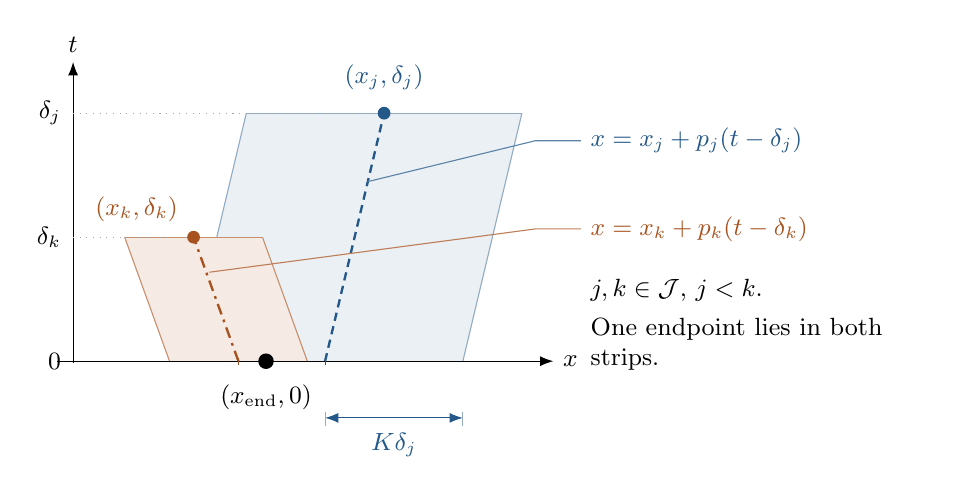
\begin{tikzpicture}[x=1cm,y=1cm,>=Latex,font=\small]
  \definecolor{fitblue}{RGB}{35,88,136}
  \definecolor{fitorange}{RGB}{168,83,31}
  \fill[fitblue!9] (-1.00,0)--(2.50,0)--(3.25,3.15)--(-0.25,3.15)--cycle;
  \draw[fitblue!50] (-1.00,0)--(-0.25,3.15) (2.50,0)--(3.25,3.15);
  \draw[fitblue!50] (-0.25,3.15)--(3.25,3.15);
  \fill[fitorange!12] (-1.225,0)--(0.525,0)--(-0.045,1.575)--(-1.795,1.575)--cycle;
  \draw[fitorange!65] (-1.225,0)--(-1.795,1.575) (0.525,0)--(-0.045,1.575);
  \draw[fitorange!65] (-1.795,1.575)--(-0.045,1.575);
  \draw[fitblue,densely dashed,line width=0.85pt] (0.75,0)--(1.50,3.15);
  \draw[fitorange,dash pattern=on 4pt off 2pt on 1pt off 2pt,line width=0.85pt]
      (-0.35,0)--(-0.92,1.575);
  \draw[->] (-2.65,0)--(3.65,0) node[right] {$x$};
  \draw[->] (-2.45,-0.02)--(-2.45,3.80) node[above] {$t$};
  \draw[black!35,dotted] (-2.45,3.15)--(1.50,3.15);
  \draw[black!35,dotted] (-2.45,1.575)--(-0.92,1.575);
  \node[left] at (-2.48,3.15) {$\delta_j$};
  \node[left] at (-2.48,1.575) {$\delta_k$};
  \node[left] at (-2.48,0) {$0$};
  \fill[fitblue] (1.50,3.15) circle (2.3pt);
  \node[above=5pt,fitblue] at (1.50,3.15) {$(x_j,\delta_j)$};
  \fill[fitorange] (-0.92,1.575) circle (2.3pt);
  \node[above left=3pt,fitorange] at (-0.92,1.575) {$(x_k,\delta_k)$};
  \fill (0,0) circle (2.8pt);
  \node[below=5pt] at (0,0) {$(x_{\rm end},0)$};
  \draw[fitblue] (0.75,-0.045)--(0.75,0.045);
  \draw[fitorange] (-0.35,-0.045)--(-0.35,0.045);
  \node[anchor=west,align=left,fitblue] (ja) at (4.00,2.80)
      {$x=x_j+p_j(t-\delta_j)$};
  \draw[fitblue!75] (ja.west)--(3.42,2.80)--(1.29,2.28);
  \node[anchor=west,align=left,fitorange] (ka) at (4.00,1.68)
      {$x=x_k+p_k(t-\delta_k)$};
  \draw[fitorange!75] (ka.west)--(3.42,1.68)--(-0.72,1.13);
  \node[anchor=west,align=left,text width=4.25cm] at (4.00,0.46)
      {$j,k\in\mathcal J$, $j<k$.\\[3pt]
       One endpoint lies in both strips.};
  \draw[fitblue,<->] (0.75,-0.72)--(2.50,-0.72)
      node[midway,below=2pt] {$K\delta_j$};
  \draw[fitblue!50] (0.75,-0.64)--(0.75,-0.82)
                        (2.50,-0.64)--(2.50,-0.82);
\end{tikzpicture}
\caption{Schematic localization at two selected scales, shown in one spatial
 direction with different horizontal and vertical units. The dashed axes
 belong to the two fitted frames; each shaded endpoint-localization strip has spatial half-width
 $K\delta_j$ or $K\delta_k$. Their time-zero sections both contain the
 same point $(x_{\rm end},0)$, expressing
 $|x_{\rm end}-x_j+p_j\delta_j|\le K\delta_j$.
 The conclusion holds for infinitely many selected indices
 $j\in\mathcal J$. The axes are separate affine fits, not a trajectory
 joining the marks.}
\label{fig:contact-localization}
\end{figure}


\begin{proof}
We first construct finite stopped walks with common expectation and error
bounds, and then localize their terminal points in the frames of their
marks.  Finally, one joint limiting law will retain the terminal point and
all marks, allowing us to select infinitely many localized contacts for the
same endpoint.

\medskip\noindent\emph{The stopped walks and their expectation bounds.}
Fix for the moment an integer $T\ge2$ and a radius $R\ge2$.  For each
$N\ge1$ choose $\epsilon_N$ to be an inverse power of two with
\begin{equation}\label{eq:contact-grid}
  0<\epsilon_N\le\frac{\delta_N}{4}.
\end{equation}
In particular, $\epsilon_N$ divides $1,T$, and every $\delta_j$ with
$j\le N$.  We will make each $\epsilon_N$ smaller if necessary, retaining
these conditions.  Write $\epsilon=\epsilon_N$ while constructing the
$N$-th walk.

Start at $z_0=z_*$.  At a state $z_n=(x_n,t_n)$ with
$\delta_N<t_n<T$ and $|x_n|<R$, choose the two steps of
\eqref{eq:dp-step-choice} and take $z_{n+1}=z_n^+$ or $z_n^-$ with equal
probabilities.  Stop on first reaching $t_n=\delta_N$, $t_n=T$, or
$|x_n|\ge R$; call this stopping index $\tau_N$.  The choices of optimizers
can be made separately at every node of the countable tree of finite
histories.  Taking independent fair signs $\xi_n\in\{-1,1\}$ to select the
steps then defines the walk and the filtration
$\mathcal F_n=\sigma(\xi_0,\ldots,\xi_{n-1})$; all velocities at step $n$
are $\mathcal F_n$-measurable.  In expressions such as $Q_-(z_n)$ below,
the velocity denotes the choice made at that history.  Before stopping,
$t_n>\delta_N\ge4\epsilon$, so the inequality \eqref{eq:dp-drift} applies.

We choose $\epsilon_N$ sufficiently small that every position up to and
including the stop lies in $\overline B_{R+1}(0)$.  Here is the uniform
localization of optimizers that permits this choice.  The sandwich for $W$
extends it continuously to $t=0$ by $W(x,0)=v(x,0)$.  The growth bounds for
$v$ and the sandwich give uniform subquadratic growth for $v$ and $W$ on
compact time intervals in $\R$ and $[0,\infty)$, respectively.  For base
points in a fixed compact box and lengths
$\ell\le1$, a quadratic cost first confines all optimizing positions for
$\Penv_\ell W$ and $\Menv_\ell v$ to a fixed spatial compact set: outside a
sufficiently large ball the cost dominates the uniform subquadratic bound,
even with the weaker coefficient corresponding to $\ell=1$.  On that compact
set the functions are bounded.  Comparing an optimizer with the zero
displacement competitor then gives $|y-x|^2/(2\ell)\le C$ there, uniformly
as $\ell\downarrow0$.  Thus the optimizing displacements tend to zero
uniformly.  Apply this to length $2\epsilon$ and base points with
$|x|\le R$, $0\le t\le T$, in a slightly larger time interval.  The
intermediate displacements used for the steps are half the full
displacements, so they can all be made at most one.  This proves the asserted
bound at stopping.  We also choose $\epsilon_N$ small enough that
\begin{equation}\label{eq:contact-start-lower}
  J_{\epsilon_N}(z_*)\ge H_*-1,
\end{equation}
which is possible by \eqref{eq:dp-J-contact}.

The time coordinate before stopping is the simple symmetric walk with step
$\epsilon$ starting at $1$.  It is stopped no later than this time walk hits
$\delta_N$ or $T$.  The latter hitting time is almost surely finite and has
finite expectation, for example by the elementary gambler's ruin formula.
The same is therefore true of $\tau_N$.  Put
\[
  \mathcal B=\overline B_{R+1}(0)\times[0,T],\qquad B=R+T+2.
\]
The upper slope bound for $v$ on boxes and \eqref{eq:dp-J-bounds} give a
constant $U_B=C L(B)^4$, independent of $N$, such that
\begin{equation}\label{eq:contact-J-upper}
  J_{\epsilon_N}(z_n)\le U_B\qquad (0\le n\le\tau_N).
\end{equation}

For any stopping time $\sigma\le\tau_N$, summing the conditional form of
\eqref{eq:dp-drift} up to $\sigma\wedge h$ gives
\begin{equation}\label{eq:contact-truncated-drift}
\begin{split}
  \mathbb E J_\epsilon(z_{\sigma\wedge h})
  &\ge J_\epsilon(z_*)\\
  &\quad+c\,\mathbb E\sum_{n<\sigma\wedge h}
          \bigl(|Q_+(z_n)-Q_0(z_n)|^2+|Q_-(z_n)-Q_0(z_n)|^2\bigr).
\end{split}
\end{equation}
For each fixed $N$, $J_\epsilon$ is continuous and bounded on the compact
box $\overline B_{R+1}(0)\times[\delta_N,T]$ containing the stopped walk.
Thus dominated convergence applies to its
term as $h\to\infty$.  Monotone convergence applies to the nonnegative sum.
We obtain, for all these stopping times,
\begin{equation}\label{eq:contact-stopped-expectation}
  \mathbb E J_\epsilon(z_\sigma)\ge J_\epsilon(z_*).
\end{equation}
Taking $\sigma=\tau_N$ in \eqref{eq:contact-truncated-drift} and using
\eqref{eq:contact-start-lower}--\eqref{eq:contact-J-upper} also gives
\begin{equation}\label{eq:contact-error-budget}
  \mathbb E\sum_{n<\tau_N}
       \bigl(|Q_+(z_n)-Q_0(z_n)|^2+|Q_-(z_n)-Q_0(z_n)|^2\bigr)
  \le B_0,\qquad B_0=C_*L(B)^4.
\end{equation}
Here $C_*$ is fixed for $v$ and independent of $N,R,T$; it absorbs the
finite number $H_*$ and the absolute constant $c$ in \eqref{eq:dp-drift}.
Both \eqref{eq:contact-stopped-expectation} and
\eqref{eq:contact-error-budget} are unconditional expectations. Together
with the upper slope bound, the lower expectation bound will give contact
and a finite terminal slope in the limit. We first use the discrepancy
bound to control horizontal-exit probabilities, both in the original
coordinates and in fitted frames.

\medskip\noindent\emph{Reaching the lower level with positive probability.}
We next show how to choose the outer cutoffs so that the walks reach
$t=\delta_N$ with probability at least $3/4$, uniformly in $N$.
Couple the time signs with
the simple symmetric walk starting at $1$ and stopped only at $0$ or $T$.
Its probability of reaching $T$ is $1/T$, which also bounds that probability
for our walk, since it may stop sooner. To control horizontal exit, we will
bound the expected maximal displacement by $C_T L(R+T+2)^2$, with $C_T$ independent
of $R$ and $N$. Markov's inequality will then make the probability of
horizontal exit tend to zero as $R\to\infty$ for fixed $T$.

The expected number of visits of the unrestricted time walk to any fixed
interior grid level is at most $CT/\epsilon$. To verify this directly,
write $q=T/\epsilon$ and identify the level with $k\in\{1,\ldots,q-1\}$.
After a visit to $k$, the
probability of reaching an endpoint before the next return is
\[
  \frac12\left(\frac1k+\frac1{q-k}\right)\ge\frac2q.
\]
This follows from the linear hitting probability for a symmetric walk on
each of the intervals $[0,k]$ and $[k,q]$. Starting from the first visit,
the expected total number of visits is at most $q/2$, by the geometric
return calculation; the probability of that first visit is at most one.
Stopping the actual walk earlier can only decrease its visit counts.
Summing this bound over levels gives
\begin{equation}\label{eq:contact-time-and-velocity-budget}
  \mathbb E(\epsilon^2\tau_N)\le CT^2,\qquad
  \mathbb E\sum_{n<\tau_N}\epsilon^2|Q_0(z_n)|^2
       \le C_T L(B)^2.
\end{equation}
For the second inequality we used Lemma~\ref{lem:dp-log-velocity} before
each step.  More explicitly, it bounds the summand velocity squared by
$C(L(B)^2+|\log t_n|^2)$, while the visit estimate gives at most
\[
  CT\epsilon\sum_{k=1}^{q-1}
           \bigl(L(B)^2+|\log(k\epsilon)|^2\bigr).
\]
This has the asserted bound.  Indeed, on $(0,1]$ the function
$|\log s|^2$ is decreasing and integrable, so its right-endpoint grid sum
times $\epsilon$ is at most its integral there; on $[1,T]$ it is bounded by
$(\log T)^2$.  The constants $C_T$ in this proof can depend on $T$ and the
fixed data, but not on $R$ or $N$.

For $n<\tau_N$ the spatial increment can be written exactly as
\[
  x_{n+1}-x_n
   =\epsilon\xi_n Q_0(z_n)
     +\epsilon\xi_n\bigl(Q_{\xi_n}(z_n)-Q_0(z_n)\bigr),
\]
where $Q_{1}=Q_+$ and $Q_{-1}=Q_-$.  Extend both kinds of increments by
zero after stopping.  The first summands are martingale differences, since
the active-step indicator and $Q_0(z_n)$ are known before the fair sign.
For a deterministic truncation in the number of steps, Doob's $L^2$ maximal
inequality and
orthogonality of these differences give an upper bound
\[
  2\left(\mathbb E\sum_{n<\tau_N}\epsilon^2|Q_0(z_n)|^2\right)^{1/2}
\]
for the expected supremum of the norm of their partial sums.  Letting the
truncation increase preserves this bound by monotone convergence of the
suprema.  On each path, the sum of the norms of the other increments is at
most
\[
  (\epsilon^2\tau_N)^{1/2}
  \left(\sum_{n<\tau_N}
       \bigl(|Q_+(z_n)-Q_0(z_n)|^2+|Q_-(z_n)-Q_0(z_n)|^2\bigr)\right)^{1/2}.
\]
Cauchy--Schwarz in expectation gives the travel inequality
\begin{equation}\label{eq:contact-travel-inequality}
\begin{split}
  \mathbb E\sup_{0\le n\le\tau_N}|x_n|
  &\le 2\left(\mathbb E\sum_{n<\tau_N}
                    \epsilon^2|Q_0(z_n)|^2\right)^{1/2}\\
  &\quad+\left(\mathbb E(\epsilon^2\tau_N)\right)^{1/2}\\
  &\qquad\times\left(\mathbb E\sum_{n<\tau_N}
       \bigl(|Q_+(z_n)-Q_0(z_n)|^2+|Q_-(z_n)-Q_0(z_n)|^2\bigr)\right)^{1/2}.
\end{split}
\end{equation}
This calculation uses only predictability of the coefficients of the fair
signs in the reference increments, including the active-step indicators,
and the pathwise bound on error lengths.  It therefore applies as well to
the displacement from the starting point of a stopped portion after a stopping
time, with its increments extended by zero outside that portion.  Equations \eqref{eq:contact-error-budget} and
\eqref{eq:contact-time-and-velocity-budget} now show that
\begin{equation}\label{eq:contact-original-travel}
  \mathbb E\sup_{0\le n\le\tau_N}|x_n|
    \le C_T\bigl(L(B)+\sqrt{B_0}\bigr)
    \le C'_T L(B)^2.
\end{equation}

The probability of a horizontal stop is at most the right side of
\eqref{eq:contact-original-travel} divided by $R$. For fixed $T$ this tends
to zero as $R\to\infty$. Choose an integer $T\ge8$, and then choose $R$
large enough that
the horizontal-stop probability is at most $1/8$, uniformly in $N$.
Fix these $T,R$ for the rest of the proof, so $B$ and $B_0$ are now fixed
finite constants.  If
\[
  \eta_N=\mathbf1_{\{t_{\tau_N}=\delta_N\}},
\]
the two preceding bounds and the definition of the stop imply
\begin{equation}\label{eq:contact-lower-hit-probability}
  \mathbb P(\eta_N=1)\ge\frac34\qquad(N\ge1).
\end{equation}
This remains true if the lower time level and the horizontal cutoff are
reached simultaneously, since that case has $\eta_N=1$.

\medskip\noindent\emph{Marks and localization in fitted frames.}
For $1\le j\le N$, let
\[
  \sigma_{j,N}=\tau_N\wedge\inf\{n\ge0:t_n=\delta_j\},\qquad
  z_j=(x_j,t_j)=z_{\sigma_{j,N}}.
\]
Thus a mark is the first point on its time level, or the terminal point if
the walk stops before that level.  The divisibility of the grid ensures
$t_j\ge\delta_j$, with equality on $\{\eta_N=1\}$.  At the time of this
mark choose a fit $(p_j,a_j)$ at $z_j$ of radius $\delta_j$.  These choices
can again be made on the countable tree of histories, so the parameters are
$\mathcal F_{\sigma_{j,N}}$-measurable.  The bound on fit parameters on boxes
gives, for a fixed constant independent of $N$,
\[
  |p_j|+|a_j|\le\Gamma_j:=C\bigl(L(B)+j\bigr),\qquad j\le N,
\]
increasing $C$ to make every $\Gamma_j\ge1$.

The cutoffs $T,R$ and the error bound $B_0$ are now fixed.  We will choose
two further cutoffs, uniformly in $j,N$, to control the terminal point in
each fitted frame.  Fix $1\le j\le N$, put $r=\delta_j$, and let
$\mathcal R_{j,N}=\{t_j=r\}$ be the event that the level $r$ is reached,
including the case where it is reached at the original stop.  This event is
$\mathcal F_{\sigma_{j,N}}$-measurable.  On it $z_j=(x_j,r)$, so we may apply
Lemma~\ref{lem:fitted-frame-covariance} pathwise with the chosen fit
$(p_j,a_j)$.  In its coordinates,
\[
  s=\frac{t}{r},\qquad
  y=\frac{x-x_j-p_j(t-r)}{r},\qquad
  \epsilon'=\frac{\epsilon_N}{r}.
\]
The transformed solution $\bar v$ is centered at $(0,1)$ and has the same
Jensen bound.  Its $\bar W$ therefore has the standing properties of
Section~\ref{sec:discrete-propagation}.  The mapped steps are optimizing
steps, and \eqref{eq:contact-velocity-covariance} gives identical squared
velocity discrepancies.  Contact at this finite mark is not needed.  The
fit and frame are known at the marking time and will be held fixed afterward.

On $\mathcal R_{j,N}$ consider the portion of the original walk from its
$j$-th mark to its stop, with the additional rule that this portion stops
on first reaching $s=M$ or $|y|\ge K$, where $M\ge2$ is an integer and
$K\ge2$.  It includes the endpoint of this additional stopping rule.  If
the original walk stopped at the mark, the portion has no steps.  A hit of
an additional cutoff simultaneous with the original stop is counted as a
hit of that additional cutoff.  On $\mathcal R_{j,N}^{\rm c}$ define the
portion to be empty as well, and assign zero to all its sums and spatial
suprema.  Let $n'$ be its number of steps, and write $\sum'$ for a sum over
its pre-step states.

The total squared velocity error on this portion, in the new frame, has the
unconditional bound
\begin{equation}\label{eq:contact-frame-error-budget}
  \mathbb E\sum'
       \bigl(|Q'_+-Q'_0|^2+|Q'_--Q'_0|^2\bigr)\le B_0.
\end{equation}
Indeed, on each path the sum is a subsum of the original sum in
\eqref{eq:contact-error-budget}, with identical summands by
\eqref{eq:contact-velocity-covariance}; on an empty portion it is zero.
This argument gives an unconditional estimate.  It makes no assertion that
the same bound holds after conditioning on a particular history at the
mark.

The time-walk estimates, in contrast, do hold conditionally on that history.
On $\mathcal R_{j,N}$ the new time starts at $s=1$ and has step
$\epsilon'=\epsilon_N/r\le1/4$, which divides $1$ and $M$.  Given
$\mathcal F_{\sigma_{j,N}}$, the subsequent signs remain fair.  The portion
is stopped no later than the unrestricted new time walk first hits $0$ or
$M$.  Its conditional expected visits to each interior level are therefore
at most $CM/\epsilon'$ by the same visit argument used above.  Before any
step of the portion, the original walk is still live, so
$s=t/r>\delta_N/r\ge4\epsilon'$.  Also $|y|<K$ and $s<M$ before the
additional stop.  Lemma~\ref{lem:dp-log-velocity} applies to the centered
$\bar v$ and its $\bar W$ uniformly, and bounds $|Q'_0|$ by
$C(L(K+M+2)+|\log s|)$.  The integrable logarithmic grid sum gives
\begin{equation}\label{eq:contact-frame-time-budget}
\begin{split}
  \mathbb E\bigl((\epsilon')^2n'\mid\mathcal F_{\sigma_{j,N}}\bigr)
       &\le CM^2\mathbf1_{\mathcal R_{j,N}},\\
  \mathbb E\left(\sum'
          (\epsilon')^2|Q'_0|^2\,\middle|\,\mathcal F_{\sigma_{j,N}}\right)
       &\le C_M L(K+M+2)^2\mathbf1_{\mathcal R_{j,N}}.
\end{split}
\end{equation}
The frame is known at the conditioning time, and the estimates of the
centered class have constants independent of that frame.  This explains the
uniformity of these conditional bounds.  Integrating them gives the same
bounds unconditionally without the indicator.

Extend the new increments by zero outside the portion.  Their reference
part is $\epsilon'\xi_nQ'_0$ and their error part is
$\epsilon'\xi_n(Q'_{\xi_n}-Q'_0)$.  The reference increments are martingale
differences after the random starting mark: the fit and reached event are
known at that mark, and on an active step the indicator and
$Q'_0=Q_0-p_j$ are $\mathcal F_n$-measurable while $\xi_n$ is still fair
given $\mathcal F_n$.  Thus the calculation of
\eqref{eq:contact-travel-inequality} applies in the primed variables.  Using
the integrated bounds from
\eqref{eq:contact-frame-time-budget} and the unconditional bound
\eqref{eq:contact-frame-error-budget}, it gives
\begin{equation}\label{eq:contact-frame-travel}
  \mathbb E\left(\sup_{\text{points of the portion}}|y|\right)
   \le C'_M\bigl(L(K+M+2)+\sqrt{B_0}\bigr).
\end{equation}
The supremum is understood to be zero for an empty portion.  In particular,
the probability that this portion reaches $|y|\ge K$ is at most the right
side of \eqref{eq:contact-frame-travel} divided by $K$.  The probability it
reaches $s=M$ is at most $1/M$: conditionally on reaching the mark, the
unrestricted symmetric time walk starting from $1$ hits $M$ before $0$ with
probability $1/M$, and an earlier stop only removes this event.

Choose a fixed integer $M\ge8$, and then choose $K$ so large that
\[
  \frac{C'_M\bigl(L(K+M+2)+\sqrt{B_0}\bigr)}{K}\le\frac18.
\]
This is possible because $B_0$ is already fixed and $L(K+M+2)/K\to0$.
On $\{\eta_N=1\}$ the $j$-th level is reached.  If neither additional
cutoff intervenes, the terminal point is in the portion and has $|y|\le K$.
Combining this observation with \eqref{eq:contact-lower-hit-probability}
and the two additional-cutoff probabilities proves, uniformly for $j\le N$,
\begin{equation}\label{eq:contact-finite-localization}
  \mathbb P\left(\eta_N=1,\quad
      |x_{\tau_N}-x_j-p_j(t_{\tau_N}-\delta_j)|\le K\delta_j\right)
       \ge\frac34-\frac18-\frac18=\frac12.
\end{equation}

\medskip\noindent\emph{One limiting law and the contact properties.}
We use one fixed compact space for all these laws.  Define
\[
  \mathcal K_j=\mathcal B\times\overline B_{\Gamma_j}(0)
                    \times[-\Gamma_j,\Gamma_j],
  \qquad
  \mathcal X=\mathcal B\times\{0,1\}\times\prod_{j=1}^{\infty}\mathcal K_j.
\]
The coordinates are the terminal point, the flag, and the marked point and
fit at each index.  This countable product of compact metric spaces is
compact and metrizable.  For indices $j>N$, fill the coordinates by any
fixed point of $\mathcal K_j$; these dummy entries need not be fits.  Let
$\mu_N$ be the law on $\mathcal X$ of the terminal point $z_{\tau_N}$, the
flag $\eta_N$, and the marked points and fits.  Compactness of the space
of probability measures on a compact metric space gives a subsequence
converging weakly to a probability law $\mu$; all subsequent limits in $N$
are along this subsequence.  Denote its coordinates by
$z_{\rm end}=(x_{\rm end},t_{\rm end})$, $\eta$, and
$(z_j,p_j,a_j)$.

Here are first the properties that pass directly to this law.  The flag is
a coordinate in a discrete space, so its probability converges and
$\mu(\eta=1)\ge3/4$.  Also the continuous nonnegative function
$\eta t_{\rm end}$ on $\mathcal X$ has integral at most $\delta_N$ under
$\mu_N$.  Its integral under $\mu$ is zero.  It follows that
$t_{\rm end}=0$ almost surely on $\{\eta=1\}$.  For each fixed $j$, the sets
$\{t_j\ge\delta_j\}$ and $\{\eta=0\}\cup\{t_j=\delta_j\}$ are closed and
have $\mu_N$-measure one for all $N\ge j$.  The closed-set direction of the
Portmanteau Theorem, $\limsup_N\mu_N(F)\le\mu(F)$, makes their
$\mu$-measures one.  Fits at the specified radius form a closed subset of
$\mathcal K_j$.  To see this without varying the sheared domain, write its
increments in \eqref{eq:limit-fit} as
\[
  \ell=\delta_j\theta,\qquad
  h=p_j\delta_j\theta+\delta_j\zeta,
  \qquad |\theta|\le1,\quad |\zeta|\le1.
\]
For each $(\theta,\zeta)$ the fitting inequality is closed in
$(z_j,p_j,a_j)$ by continuity of $v$, and their intersection over this
fixed compact set of increments is closed.  Portmanteau therefore also
passes the fitting property to $\mu$.  Taking the intersection of the
resulting full-measure sets for all $j$, we have
\begin{equation}\label{eq:contact-mark-limit}
\begin{gathered}
  t_{\rm end}=0\text{ on }\{\eta=1\},\qquad
  t_j\ge\delta_j\text{ and }t_j=\delta_j\text{ on }\{\eta=1\},\\
  (p_j,a_j)\text{ is a fit at }z_j\text{ of radius }\delta_j
       \quad\text{for every }j,
\end{gathered}
\end{equation}
almost surely.

Two further properties come from the expectation bounds:
\begin{equation}\label{eq:contact-limit-properties}
  H_v(z_{\rm end})>-\infty,\qquad W(z_j)=v(z_j)\quad(j\ge1)
  \qquad\text{almost surely under }\mu.
\end{equation}
For the first, fix $\ell>0$ and set
\[
  \Phi_\ell(z)=\frac12\bigl(\Senv^+_\ell v(z)+\Senv^-_\ell v(z)\bigr).
\]
This is a finite continuous function on $\mathcal B$.  For all sufficiently
large $N$, $\epsilon_N\le\ell$, and monotonicity of both slopes with respect
to their length and \eqref{eq:dp-J-bounds} give
$J_{\epsilon_N}\le\Phi_\ell$.  Apply
\eqref{eq:contact-stopped-expectation} at $\tau_N$ and pass to the weak limit
using this fixed continuous function and \eqref{eq:dp-J-contact}.  The
result is
\begin{equation}\label{eq:contact-terminal-slopes}
  \int\Phi_\ell(z_{\rm end})\,d\mu\ge H_*\qquad(\ell>0).
\end{equation}
Take a decreasing sequence $\ell_h\downarrow0$ with $\ell_h\le1$.  The
functions $\Phi_{\ell_h}$ decrease to $H_v$ pointwise, because the two slope
limits agree for $v$.  Their uniform upper bound on $\mathcal B$ is $U_B$
after increasing its fixed constant.  Hence
$U_B-\Phi_{\ell_h}(z_{\rm end})$ are nonnegative and increase to
$U_B-H_v(z_{\rm end})$.  Monotone convergence and
\eqref{eq:contact-terminal-slopes} give
\[
  \int\bigl(U_B-H_v(z_{\rm end})\bigr)\,d\mu\le U_B-H_*<\infty.
\]
The integrand would be infinite where $H_v=-\infty$, proving the first
claim of \eqref{eq:contact-limit-properties}.

For the contact claim fix $j$ and let $\nu_N^j$ and $\nu^j$ be the marginals
of $\mu_N$ and $\mu$ for the marked point $z_j$.  They converge weakly.
Suppose that $\nu^j$ gives positive mass to $\{v-W>0\}$.  All these limit
marks have $t\ge\delta_j$.  Since $v-W$ is continuous and nonnegative for
$t>0$, there is $\alpha>0$ such that the relatively open set
\[
  U=\{(x,t)\in\mathcal B:t>\delta_j/2,\ v(x,t)-W(x,t)>\alpha\}
\]
has $\nu^j(U)>0$ and its closure is contained in
$\{t\ge\delta_j/2,\ v-W\ge\alpha\}$.  For example, first choose $\alpha$
with positive mass where $v-W>2\alpha$.  The zero-length continuity of the
quadratic envelopes is uniform on this compact closure.  Thus
\eqref{eq:dp-contact-gap} gives
\[
  2\epsilon_NJ_{\epsilon_N}(z)
   \le-\frac{\alpha}{2}
\]
on $U$ for all sufficiently large $N$.  In particular,
$J_{\epsilon_N}\le-\alpha/(4\epsilon_N)$ on $U$.  By the open-set direction
of Portmanteau, $\nu^j(U)\le\liminf_N\nu_N^j(U)$, so these probabilities
are bounded below by a fixed positive number for large $N$.  The uniform
upper bound \eqref{eq:contact-J-upper} on all marks and
\eqref{eq:contact-stopped-expectation} at $\sigma_{j,N}$ would then give
\[
  J_{\epsilon_N}(z_*)\le\int J_{\epsilon_N}\,d\nu_N^j
  \le-\frac{\alpha}{4\epsilon_N}\nu_N^j(U)
      +U_B\bigl(1-\nu_N^j(U)\bigr)\longrightarrow-\infty.
\]
This contradicts \eqref{eq:dp-J-contact}.  Thus $W(z_j)=v(z_j)$ almost
surely.  A countable intersection proves this simultaneously for all $j$.
The derivation of \eqref{eq:contact-limit-properties} used unconditional
expectations; it does not require conditioning on the flag.

For each fixed $j$ define the subset of $\mathcal X$
\[
  E_j=\left\{\eta=1,\quad
      |x_{\rm end}-x_j-p_j(t_{\rm end}-\delta_j)|\le K\delta_j\right\}.
\]
This event retains the actual terminal time in the prelimit laws.
It is closed: the flag condition is closed and the norm is a continuous
function of the terminal point, the $j$-th marked point, and $p_j$.
Equation~\eqref{eq:contact-finite-localization} gives
$\mu_N(E_j)\ge1/2$ whenever $N\ge j$.  The
closed-set Portmanteau inequality has the direction
\[
  \mu(E_j)\ge\limsup_{N\to\infty}\mu_N(E_j)\ge\frac12.
\]
These events need not be independent.  For every $h$ their tail union has
measure at least $1/2$, since it contains each $E_j$ with $j\ge h$.  Continuity of
probability from above therefore gives
\[
  \mu\left(\limsup_{j\to\infty}E_j\right)
   =\lim_{h\to\infty}\mu\left(\bigcup_{j\ge h}E_j\right)\ge\frac12.
\]
Choose one outcome in this limsup event and in the full-measure sets of
\eqref{eq:contact-mark-limit}--\eqref{eq:contact-limit-properties}.  Every
$E_j$ includes $\eta=1$, so this outcome has $t_{\rm end}=0$ and
$t_j=\delta_j$ for every $j$.  It belongs to $E_j$ for an infinite set of
indices, at each of which its localization inequality is
\[
  |x_{\rm end}-x_j+p_j\delta_j|\le K\delta_j.
\]
The same outcome has a finite common slope at the endpoint, contact at all
the marks, and the indicated fits.  Its endpoint and the infinite set of
these marks establish \eqref{eq:contact-propagation-conclusion}.
\end{proof}

\section{Rigidity of the final limit}\label{sec:rigidity}

The propagation result produces contacts at shrinking scales near one terminal point. The finite slope at that point makes the final limit have constant forward and backward envelope slopes at every length. We first show why this forces an affine function.

\begin{lemma}[Rigidity from constant envelope slopes]\label{lem:slope-rigidity}
Let $v\in\Aclass_{m,C_0}$, with the class and envelopes defined in Section~\ref{sec:limiting-tools}. Suppose that for some $(b,t_0)\in\R^m\times\R$ and $B\in\R$,
\begin{equation}\label{eq:constant-envelope-slopes}
  \Senv_\ell^+v(b,t_0)=\Senv_\ell^-v(b,t_0)=B
       \qquad\text{for every }\ell>0.
\end{equation}
Then $v$ is affine.
\end{lemma}

\begin{proof}
Translate $(b,t_0)$ to $(0,0)$ and subtract the value there; write $V$ for the resulting function. These changes preserve the class and the envelope slopes. The forward equality in \eqref{eq:constant-envelope-slopes} gives $\Penv_tV(0,0)=Bt$ for $t>0$, and therefore
\begin{equation}\label{eq:future-paraboloid}
  V(y,t)\le Bt+\frac{|y|^2}{2t}\qquad(t>0).
\end{equation}

Fix any $(x,t)\in\R^m\times\R$. At a large length $\ell$, a maximizing position $y_\ell$ for $\Penv_\ell V(x,t)$ satisfies
\begin{equation}\label{eq:rigidity-optimizer-bound}
  |y_\ell|\le C_{x,t}\ell(1+\log\ell)^2.
\end{equation}
This is the optimizer estimate from Section~\ref{sec:limiting-tools}, applied on a box of size comparable to $\ell$; the translated function has the same growth estimates with constants depending on a fixed value and fit. Explicitly, if the displacement is $b_\ell\ell$ with $b_\ell\ge2$, comparison with zero displacement and the bound $|V(y,s)|\le C K(1+\log K)^2$ on boxes of size $K$ give
\[
  b_\ell\le C_{x,t}(1+\log\ell+\log b_\ell)^2.
\]
Absorbing the logarithmic term in $b_\ell$ gives $b_\ell\le C_{x,t}'(1+\log\ell)^2$, which proves \eqref{eq:rigidity-optimizer-bound}.

For $\ell$ sufficiently large, $t+\ell>0$, so \eqref{eq:future-paraboloid} applies at the optimizer. The difference between the two quadratic costs is
\begin{align*}
  \frac{|y_\ell|^2}{2(t+\ell)}-\frac{|y_\ell-x|^2}{2\ell}
  &=-\frac{t|y_\ell|^2}{2\ell(t+\ell)}
       +\frac{x\cdot y_\ell}{\ell}-\frac{|x|^2}{2\ell}\\
  &=O_{x,t}\bigl((1+\log\ell)^4\bigr)=o(\ell)
\end{align*}
by \eqref{eq:rigidity-optimizer-bound}. Consequently
\[
  \limsup_{\ell\to\infty}\Senv_\ell^+V(x,t)\le B.
\]
The forward slopes are nondecreasing in $\ell$ by Lemma~\ref{lem:envelope-slopes}. Thus $\Senv_\ell^+V(x,t)\le B$ for every $\ell>0$. Evaluating the envelope at any competitor gives the global directed comparison
\begin{equation}\label{eq:directed-comparison}
  V(y,t+\ell)-V(x,t)\le B\ell+\frac{|y-x|^2}{2\ell}
       \qquad(x,y\in\R^m,\ t\in\R,\ \ell>0).
\end{equation}

The envelopes are attained by Lemma~\ref{lem:quadratic-envelopes}. At the origin, \eqref{eq:constant-envelope-slopes} therefore supplies, for every $\ell,r>0$, a forward equality point $(\ell q_+,\ell)$ and a backward equality point $(-r q_-,-r)$, with
\[
  V(\ell q_+,\ell)=B\ell+\tfrac12\ell|q_+|^2,
  \qquad V(-r q_-,-r)=-Br-\tfrac12r|q_-|^2.
\]
Apply \eqref{eq:directed-comparison} directly from the backward point to the forward point. After canceling $B(\ell+r)$, it gives
\[
  0\ge \frac{\ell|q_+|^2+r|q_-|^2}{2}
       -\frac{|\ell q_++r q_-|^2}{2(\ell+r)}
    =\frac{\ell r}{2(\ell+r)}|q_+-q_-|^2.
\]
Hence every forward and backward equality velocity is one vector $q$, independent of all lengths and choices. We have
\[
  V(qs,s)=(B+|q|^2/2)s\qquad(s\in\R).
\]
Let $A(x,t)=q\cdot x+(B-|q|^2/2)t$. Comparing $(x,t)$ to a point $(qs,s)$ on this line in \eqref{eq:directed-comparison} yields
\[
  V(x,t)\le A(x,t)+\frac{|x-qt|^2}{2(t-s)}\quad(s<t),
  \qquad
  V(x,t)\ge A(x,t)-\frac{|x-qt|^2}{2(s-t)}\quad(s>t).
\]
Letting $s\to-\infty$ and $s\to+\infty$ proves $V=A$.
\end{proof}

\begin{proof}[Proof of Theorem~\ref{thm:liouville}]
Suppose that the class contains a nonaffine function. Proposition~\ref{prop:envelope-contact} supplies a centered solution $v$, a number $\kappa>0$, and its subsolution envelope
\[
  W(x,t)=\Cenv_t v(x,t)-\kappa^2t/2\qquad(t>0)
\]
with the stated contact and finite-slope properties. Proposition~\ref{prop:contact-propagation} supplies a point $x_{\mathrm{end}}$, infinitely many indices $j$ with $r_j=2^{-j}$, contacts $(x_j,r_j)$, and fits $(p_j,a_j)$ there of radius $r_j$, such that
\begin{equation}\label{eq:final-contact-data}
  H_v(x_{\mathrm{end}},0)>-\infty,\qquad
  W(x_j,r_j)=v(x_j,r_j),\qquad
  |x_{\mathrm{end}}-x_j+p_jr_j|\le K r_j
\end{equation}
for one finite $K$.

Apply Lemma~\ref{lem:fitted-frame-covariance} at each of these marks, and denote the transformed functions by $\bar v_j$. Their images of $(x_{\mathrm{end}},0)$ are $(b_j,0)$, where
\[
  b_j=\frac{x_{\mathrm{end}}-x_j+p_jr_j}{r_j}.
\]
These vectors are bounded by \eqref{eq:final-contact-data}. Every $\bar v_j$ has value zero and the zero fit of radius one at $(0,1)$. Lemma~\ref{lem:fit-compactness} gives a subsequence for which $\bar v_j\to v_\infty$ locally uniformly and $b_j\to b$. The uniform growth bounds also give convergence of the forward and backward envelopes at each fixed positive length, by Lemma~\ref{lem:quadratic-envelopes}.

The slope covariance \eqref{eq:fitted-slope-covariance} gives
\[
  \Senv_\ell^\pm\bar v_j(b_j,0)
    =\Senv_{r_j\ell}^\pm v(x_{\mathrm{end}},0)-a_j
       \qquad(\ell>0).
\]
Let $B=\Senv_1^+v_\infty(b,0)$, which is finite. For each fixed $\ell>0$, subtract the equality with the forward slope at length one:
\begin{align*}
  \Senv_\ell^\pm\bar v_j(b_j,0)-\Senv_1^+\bar v_j(b_j,0)
   &=\Senv_{r_j\ell}^\pm v(x_{\mathrm{end}},0)
        -\Senv_{r_j}^+v(x_{\mathrm{end}},0)\\
   &\longrightarrow0.
\end{align*}
The limit is zero because both unshifted slopes tend to the same finite value $H_v(x_{\mathrm{end}},0)$. Passing to the limit on the left gives
\[
  \Senv_\ell^+v_\infty(b,0)=\Senv_\ell^-v_\infty(b,0)=B
       \qquad(\ell>0).
\]
This argument uses each fixed length along the same locally convergent subsequence; no convergence of the individual shifts $a_j$ is required. Lemma~\ref{lem:slope-rigidity} now makes $v_\infty$ affine.

The contacts retain a positive envelope gap. By \eqref{eq:contact-barycentric-gap} at the contacts in \eqref{eq:final-contact-data} and the gap covariance \eqref{eq:contact-W-covariance},
\[
  \Cenv_1\bar v_j(0,1)-\bar v_j(0,1)=\kappa^2/2.
\]
Lemma~\ref{lem:barycentric-envelope} passes this identity to the locally uniform limit with its uniform growth bound. Thus
\[
  \Cenv_1v_\infty(0,1)-v_\infty(0,1)=\kappa^2/2>0.
\]
For an affine function, the average of its values at any configuration is its value at the barycenter, so the nonnegative variance penalty makes $\Cenv_1v_\infty=v_\infty$. This contradiction proves Theorem~\ref{thm:liouville}. The reduction in Section~\ref{sec:reduction} then proves Theorem~\ref{thm:main}.
\end{proof}

\begin{thebibliography}{99}

\bibitem{ArmstrongCrandallJulinSmart2011}
S.~N.~Armstrong, M.~G.~Crandall, V.~Julin, and C.~K.~Smart,
\emph{Convexity criteria and uniqueness of absolutely minimizing functions},
Arch. Ration. Mech. Anal. \textbf{200} (2011), no.~2, 405--443.
\href{https://doi.org/10.1007/s00205-010-0348-0}{doi:10.1007/s00205-010-0348-0}.

\bibitem{ArmstrongSmart2010}
S.~N.~Armstrong and C.~K.~Smart,
\emph{An easy proof of Jensen's theorem on the uniqueness of infinity harmonic functions},
Calc. Var. Partial Differential Equations \textbf{37} (2010), nos.~3--4, 381--384.
\href{https://doi.org/10.1007/s00526-009-0267-9}{doi:10.1007/s00526-009-0267-9}.

\bibitem{Aronsson1967}
G.~Aronsson,
\emph{Extension of functions satisfying Lipschitz conditions},
Ark. Mat. \textbf{6} (1967), 551--561.
\href{https://doi.org/10.1007/BF02591928}{doi:10.1007/BF02591928}.

\bibitem{Aronsson1984}
G.~Aronsson,
\emph{On certain singular solutions of the partial differential equation
  $u_x^2u_{xx}+2u_xu_yu_{xy}+u_y^2u_{yy}=0$},
Manuscripta Math. \textbf{47} (1984), nos.~1--3, 133--151.
\href{https://doi.org/10.1007/BF01174590}{doi:10.1007/BF01174590}.

\bibitem{Brustad2026}
K.~K.~Brustad,
\emph{Infinity-harmonic functions in the plane: Regularity by injectivity},
preprint, June 6, 2026,
\href{https://arxiv.org/abs/2606.08257v1}{arXiv:2606.08257v1}.

\bibitem{CrandallEvans2001}
M.~G.~Crandall and L.~C.~Evans,
\emph{A remark on infinity harmonic functions},
Electron. J. Differential Equations Conf. \textbf{6} (2001), 123--129.
\href{https://ejde.math.txstate.edu/conf-proc/06/c6/crandall.pdf}{Journal PDF}.

\bibitem{CrandallEvansGariepy2001}
M.~G.~Crandall, L.~C.~Evans, and R.~F.~Gariepy,
\emph{Optimal Lipschitz extensions and the infinity Laplacian},
Calc. Var. Partial Differential Equations \textbf{13} (2001), no.~2, 123--139.
\href{https://doi.org/10.1007/s005260000065}{doi:10.1007/s005260000065}.

\bibitem{CIL1992}
M.~G.~Crandall, H.~Ishii, and P.-L.~Lions,
\emph{User's guide to viscosity solutions of second order partial differential equations},
Bull. Amer. Math. Soc. (N.S.) \textbf{27} (1992), no.~1, 1--67.
\href{https://doi.org/10.1090/S0273-0979-1992-00266-5}{doi:10.1090/S0273-0979-1992-00266-5}.

\bibitem{EvansSavin2008}
L.~C.~Evans and O.~Savin,
\emph{$C^{1,\alpha}$ regularity for infinity harmonic functions in two dimensions},
Calc. Var. Partial Differential Equations \textbf{32} (2008), no.~3, 325--347.
\href{https://doi.org/10.1007/s00526-007-0143-4}{doi:10.1007/s00526-007-0143-4}.

\bibitem{EvansSmart2011}
L.~C.~Evans and C.~K.~Smart,
\emph{Everywhere differentiability of infinity harmonic functions},
Calc. Var. Partial Differential Equations \textbf{42} (2011), nos.~1--2, 289--299.
\href{https://doi.org/10.1007/s00526-010-0388-1}{doi:10.1007/s00526-010-0388-1}.

\bibitem{Jensen1993}
R.~Jensen,
\emph{Uniqueness of Lipschitz extensions: minimizing the sup norm of the gradient},
Arch. Ration. Mech. Anal. \textbf{123} (1993), no.~1, 51--74.
\href{https://doi.org/10.1007/BF00386368}{doi:10.1007/BF00386368}.

\bibitem{PengZhangZhou2025}
F.~Peng, Y.~R.-Y.~Zhang, and Y.~Zhou,
\emph{Regularity from $p$-harmonic potentials to $\infty$-harmonic potentials in convex rings},
Proc. Lond. Math. Soc. (3) \textbf{130} (2025), no.~6, article e70062.
\href{https://doi.org/10.1112/plms.70062}{doi:10.1112/plms.70062}.

\bibitem{PeresSchrammSheffieldWilson2009}
Y.~Peres, O.~Schramm, S.~Sheffield, and D.~B.~Wilson,
\emph{Tug-of-war and the infinity Laplacian},
J. Amer. Math. Soc. \textbf{22} (2009), no.~1, 167--210.
\href{https://doi.org/10.1090/S0894-0347-08-00606-1}{doi:10.1090/S0894-0347-08-00606-1}.

\bibitem{Savin2005}
O.~Savin,
\emph{$C^1$ regularity for infinity harmonic functions in two dimensions},
Arch. Ration. Mech. Anal. \textbf{176} (2005), no.~3, 351--361.
\href{https://doi.org/10.1007/s00205-005-0355-8}{doi:10.1007/s00205-005-0355-8}.

\bibitem{Xu2026}
K.~Xu,
\emph{Infinity-harmonic functions and inverse mean curvature flow clusters},
preprint, July 7, 2026,
\href{https://arxiv.org/abs/2607.06698v1}{arXiv:2607.06698v1}.

\end{thebibliography}


\end{document}
